\documentclass[11pt,twoside,a4paper]{book}  
% definice dokumentu
\usepackage[czech, slovak, english]{babel}
\usepackage[T1]{fontenc} 				% pouzije EC fonty 
\usepackage[utf8]{inputenc} 			% utf8 kódování vstupu 
\usepackage[square, numbers]{natbib}	% sazba pouzite literatury
\usepackage{indentfirst} 				% 1. odstavec jako v cestine, pro práci v aj možno zakomentovat
\usepackage{fancyhdr}					% tisk hlaviček a patiček stránek
\usepackage{nomencl} 					% umožňuje snadno definovat zkratky a jejich seznam
\usepackage{float}
\usepackage{amsmath}
\usepackage{longtable}

% Psani definic
\usepackage{makeidx}
\usepackage{amsthm}

\usepackage{pdfpages}

\theoremstyle{definition}
\newtheorem{definice}{Definícia}[section]

%%%%%%%%%%%%%%%%%%%%%%%%%%%%%%%%%%%%%%%%%%%%%%%%%%%%%%%%%%%%%%%
% informace o práci
\newcommand\WorkTitle{Lexikální analyzátor dialektu dotazovacího jazyka databáze MySQL pro zachytávání změn v databázi}		% název
\newcommand\FirstandFamilyName{Bc. Roman Kuchár}															% autor
\newcommand\Supervisor{Ing. Jiří Pechanec}															% vedoucí

\newcommand\TypeOfWork{Diplomová práca}	% typ práce [Diplomová práce | Bakalářská práce | Bachelor's Project | Master's Thesis ]	

% Nastavte následují podle vašeho oboru a programu (pomoc hledejte na http://www.fel.cvut.cz/cz/education/bk/prehled.html)								
\newcommand\StudProgram{Otevřená informatika, Magisterský}					% program
\newcommand\StudBranch{Softwarové inženýrství}           					% obor

%%%%%%%%%%%%%%%%%%%%%%%%%%%%%%%%%%%%%%%%%%%%%%%%%%%%%%%%%%%%%%%
% minimální importy
\usepackage{graphicx}					% pro vkládání obrázků
\usepackage{k336_thesis_macros} 		% specialni makra pro formatovani DP a BP
\usepackage[
pdftitle={\WorkTitle},				% nastaví v informacích o pdf název
pdfauthor={\FirstandFamilyName},	% nastaví v informacích o pdf autora
colorlinks=false,					% před tiskem doporučujeme nastavit na false, aby odkazy a url nebyly šedé při ČB tisku
breaklinks=true,
urlcolor=red,
citecolor=blue,
linkcolor=blue,
unicode=true,
]
{hyperref}								% pro zobrazování "prokliknutelných" linků 

% rozšiřující importy
\usepackage{listings} 			%slouží pro tisk zdrojových kódů se syntax higlighting
\usepackage{algorithmicx} 		%slouží pro zápis algoritmů
\usepackage{algpseudocode} 		%slouží pro výpis pseudokódu

%%%%%%%%%%%%%%%%%%%%%%%%%%%%%%%%%%%%%%%%%%%%%%%%%%%%%%%%%%%%%%%
% příkazy šablony
\makenomenclature								% při překladu zajistí vytvoření pracovního souboru se seznamem zkratek

\let\oldUrl\url									% url adresy budou zobrazeny: <url> 
\renewcommand\url[1]{<\texttt{\oldUrl{#1}}>}

%%%%%%%%%%%%%%%%%%%%%%%%%%%%%%%%%%%%%%%%%%%%%%%%%%%%%%%%%%%%%%%
% vaše vlastní příkazy
\newcommand*{\nomExpl}[2]{#2 (#1)\nomenclature{#1}{#2}} 	% usnadňuje zápis zkratek : Slova ke Zkrácení (SZ)
\newcommand*{\nom}[2]{#1\nomenclature{#1}{#2}} 			% usnadňuje zápis zkratek : SZ

%%%%%%%%%%%%%%%%%%%%%%%%%%%%%%%%%%%%%%%%%%%%%%%%%%%%%%%%%%%%%%%
% define custom language types
\usepackage{color}
\usepackage{soul}
\usepackage{xparse}


\definecolor{editorRed}{RGB}{199, 37, 78}
\definecolor{editorLightPink}{RGB}{249, 242, 244}

\definecolor{editorLightGray}{cmyk}{0.05, 0.05, 0.05, 0.1}
\definecolor{editorGray}{cmyk}{0.6, 0.55, 0.55, 0.2}
\definecolor{editorPurple}{cmyk}{0.5, 1, 0, 0}
\definecolor{editorWhite}{cmyk}{0, 0, 0, 0}
\definecolor{editorBlack}{cmyk}{1, 1, 1, 1}
\definecolor{editorOrange}{cmyk}{0, 0.8, 1, 0}
\definecolor{editorBlue}{rgb}{0, 0, 1}
\definecolor{editorPink}{cmyk}{0, 1, 0, 0}

\definecolor{pblue}{rgb}{0,0,0.5}
\definecolor{pgreen}{rgb}{0,0.5,0}

\definecolor{maroon}{rgb}{0.5,0,0}

\NewDocumentCommand\inlinecode{v}{\sethlcolor{editorLightPink}{\color{editorRed}\hl{\mbox{#1}}}}

\lstset{
%   basicstyle=\ttfamily,
  columns=fullflexible,
  frame=single,
  numbers=left,
  stepnumber=1,
%   linewidth=14cm,
  breaklines=true,
  postbreak=\mbox{\textcolor{editorGray}{$\hookrightarrow$}\space},
}

\lstdefinelanguage{Java2}{language=Java,
  showspaces=false,
  showtabs=false,
  breaklines=true,
  showstringspaces=false,
  breakatwhitespace=true,
  commentstyle=\color{pgreen},
  keywordstyle=\color{pblue},
  stringstyle=\color{editorPurple},
  basicstyle=\ttfamily,
  basicstyle=\small,
  moredelim=[il][\textcolor{editorGray}]{$$},
  moredelim=[is][\textcolor{editorGray}]{\%\%}{\%\%}
}

\lstdefinelanguage{XML}
{
  basicstyle=\ttfamily,
  morestring=[s]{"}{"},
  morecomment=[s]{?}{?},
  morecomment=[s]{!--}{--},
  commentstyle=\color{pgreen},
  moredelim=[s][\color{editorBlack}]{>}{<},
  moredelim=[s][\color{editorRed}]{\ }{=},
  stringstyle=\color{editorBlue},
  identifierstyle=\color{maroon},
  numbers = left
}

\lstdefinelanguage{MySQL}
{
	language=SQL,
    morekeywords={AUTO_INCREMENT, REFERENCES,IF},
    morecomment=[l]{\#},
    morestring=[b]",
    commentstyle=\color{pgreen}\ttfamily,
    keywordstyle=\color{pblue}\bfseries,
  	stringstyle=\color{editorPurple}\ttfamily,
    literate=*{0}{{\textcolor{editorBlue}{0}}}{1}%
         {1}{{\textcolor{editorBlue}{1}}}{1}%
         {2}{{\textcolor{editorBlue}{2}}}{1}%
         {3}{{\textcolor{editorBlue}{3}}}{1}%
         {4}{{\textcolor{editorBlue}{4}}}{1}%
         {5}{{\textcolor{editorBlue}{5}}}{1}%
         {6}{{\textcolor{editorBlue}{6}}}{1}%
         {7}{{\textcolor{editorBlue}{7}}}{1}%
         {8}{{\textcolor{editorBlue}{8}}}{1}%
         {9}{{\textcolor{editorBlue}{9}}}{1}%
         {.0}{{\textcolor{editorBlue}{.0}}}{1}% Following is to ensure that only periods
         {.1}{{\textcolor{editorBlue}{.1}}}{1}% followed by a digit are changed.
         {.2}{{\textcolor{editorBlue}{.2}}}{1}%
         {.3}{{\textcolor{editorBlue}{.3}}}{1}%
         {.4}{{\textcolor{editorBlue}{.4}}}{1}%
         {.5}{{\textcolor{editorBlue}{.5}}}{1}%
         {.6}{{\textcolor{editorBlue}{.6}}}{1}%
         {.7}{{\textcolor{editorBlue}{.7}}}{1}%
         {.8}{{\textcolor{editorBlue}{.8}}}{1}%
         {.9}{{\textcolor{editorBlue}{.9}}}{1}%
         {\ }{{ }}{1}% handle the space
         ,%
         sensitive=true
}

\lstdefinelanguage{JavaScript}{
  keywords={break, case, catch, continue, debugger, default, delete, do, else, finally, for, function, if, in, instanceof, new, return, switch, this, throw, try, typeof, var, void, while, with, null},
  morecomment=[l]{//},
  morecomment=[s]{/*}{*/},
  morestring=[b]',
  morestring=[b]",
  commentstyle=\color{pgreen}\ttfamily,
  keywordstyle=\color{editorOrange}\bfseries,
  stringstyle=\color{editorPurple}\ttfamily,
  literate=*{0}{{\textcolor{editorBlue}{0}}}{1}%
         {1}{{\textcolor{editorBlue}{1}}}{1}%
         {2}{{\textcolor{editorBlue}{2}}}{1}%
         {3}{{\textcolor{editorBlue}{3}}}{1}%
         {4}{{\textcolor{editorBlue}{4}}}{1}%
         {5}{{\textcolor{editorBlue}{5}}}{1}%
         {6}{{\textcolor{editorBlue}{6}}}{1}%
         {7}{{\textcolor{editorBlue}{7}}}{1}%
         {8}{{\textcolor{editorBlue}{8}}}{1}%
         {9}{{\textcolor{editorBlue}{9}}}{1}%
         {.0}{{\textcolor{editorBlue}{.0}}}{1}% Following is to ensure that only periods
         {.1}{{\textcolor{editorBlue}{.1}}}{1}% followed by a digit are changed.
         {.2}{{\textcolor{editorBlue}{.2}}}{1}%
         {.3}{{\textcolor{editorBlue}{.3}}}{1}%
         {.4}{{\textcolor{editorBlue}{.4}}}{1}%
         {.5}{{\textcolor{editorBlue}{.5}}}{1}%
         {.6}{{\textcolor{editorBlue}{.6}}}{1}%
         {.7}{{\textcolor{editorBlue}{.7}}}{1}%
         {.8}{{\textcolor{editorBlue}{.8}}}{1}%
         {.9}{{\textcolor{editorBlue}{.9}}}{1}%
         {\ }{{ }}{1}% handle the space
         ,%
         sensitive=true
}

%%%%%%%%%%%%%%%%%%%%%%%%%%%%%%%%%%%%%%%%%%%%%%%%%%%%%%%%%%%%%%%

\renewcommand{\lstlistingname}{Ukážka}% Listing -> Příklad
\renewcommand{\lstlistlistingname}{Zoznam ukážok}% List of Listings -> List of Algorithms

%%%%%%%%%%%%%%%%%%%%%%%%%%%%%%%%%%%%%%%%%%%%%%%%%%%%%%%%%%%%%%%
% vlastní dokument
%%%%%%%%%%%%%%%%%%%%%%%%%%%%%%%%%%%%%%%%%%%%%%%%%%%%%%%%%%%%%%%
\begin{document}
	
	%%%%%%%%%%%%%%%%%%%%%%%%%% 
	% nastavení jazyka, kterým je práce psána
	\selectlanguage{slovak}	% podle jazyka práce nastavte na [czech | english]
	\translate				% nastaví české nebo anglické popisy (např. katedra -> department); viz k336_thesis_macros

	%%%%%%%%%%%%%%%%%%%%%%%%%%    
	% Poznamky ke kompletaci prace
	% Nasledujici pasaz uzavrenou v {} ve sve praci samozrejme 
	% zakomentujte nebo odstrante. 
	% Ve vysledne svazane praci bude nahrazena skutecnym 
	% oficialnim zadanim vasi prace.
	
%     {
	\pagenumbering{roman} \cleardoublepage \thispagestyle{empty}
	\chapter*{Na tomto místě bude oficiální zadání vaší práce}
	\begin{itemize}
		\item Toto zadání je podepsané děkanem a vedoucím katedry,
		\item musíte si ho vyzvednout na studijním oddělení Katedry počítačů na Karlově náměstí,
		\item v jedné odevzdané práci bude originál tohoto zadání (originál zůstává po obhajobě na katedře),
		\item ve druhé bude na stejném místě neověřená kopie tohoto dokumentu (tato se vám vrátí po obhajobě).
	\end{itemize}
	\newpage
	}
    
    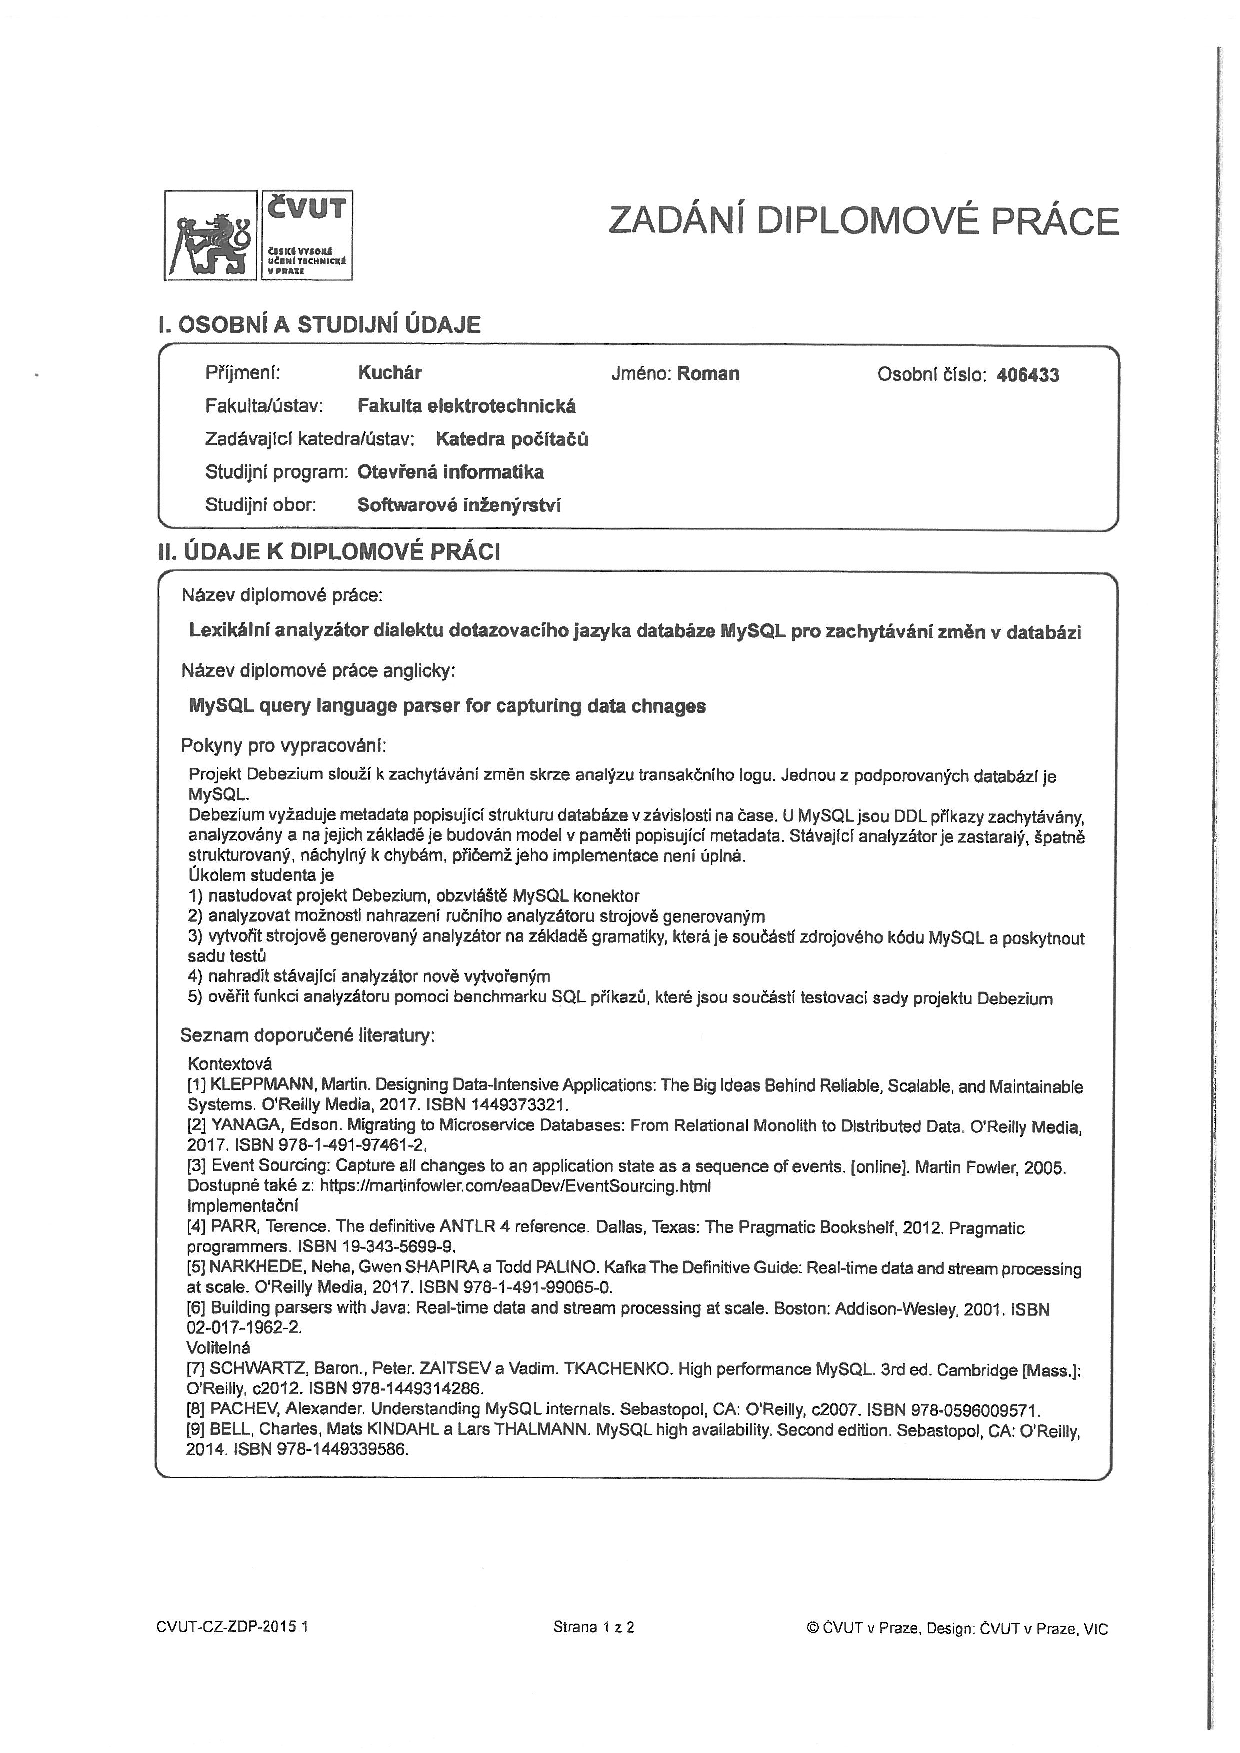
\includepdf[pages=1]{zadani_bez_podpisu.pdf}
    \includepdf[pages=2]{zadani_bez_podpisu.pdf}

	%%%%%%%%%%%%%%%%%%%%%%%%%%    
	% Titulni stranka / Title page 
	\coverpagestarts

		%%%%%%%%%%%%%%%%%%%%%%%%%%%    
	% Poděkovani / Acknowledgements 

	\acknowledgements
	\noindent
% 	Zde můžete napsat své poděkování, pokud chcete a máte komu děkovat.
Ďakujem vľtkým ale najmä sám sebe.

	
% 	%%%%%%%%%%%%%%%%%%%%%%%%%%%   
	% Prohlášení / Declaration 

	\declaration{V~Prahe dňa 20.\,5.\,2018}
% 	%\declaration{In Kořenovice nad Bečvárkou on May 15, 2008}


	%%%%%%%%%%%%%%%%%%%%%%%%%%%%    
	% Abstrakt / Abstract 
 
	\abstractpage
    

% 	Translation of Czech abstract into English.
	Project Debezium is distributed platform for change data capture in database systems. One of supported databases is MySQL, where Debezium needs meta-data for describing of the database structure. These meta-data are acquired by analysis of DDL statements, which has to be parsed. This thesis deals with the possibilities of generating the syntactic analyzers necessary to modify the in-memory model, which describes the database structure. One part of this thesis is the design and implementation of generated parser, which will replace the existing, hand written, solution in Debezium project.
   % Prace v cestine musi krome abstraktu v anglictine obsahovat i
	% abstrakt v cestine.
	\vglue60mm

	\noindent{\Huge \textbf{Abstrakt}}
	\vskip 2.75\baselineskip

	\noindent
    Projekt Debezium je distrubuovaná platforma na zachytávanie zmenených dát v databázových systémoch. Jednou z podporovaných databází je MySQL, pri ktorej Debezium potrebuje metadáta popisujúce štruktúru databázy. Tieto metadáta sú získavané na základe analýzy DDL dotazov, ktoré je nutné sparsovať. Táto práca sa zaoberá možnosťami generovania syntaktických analyzátorov potrebných na úpravu modelu uloženého v pamäti, ktorý popisuje štruktúru databázy. Súčasťou práce je návrh a implementácia generovaného syntaktického analyzátora, ktorý nahradí existujúce, ručne napísané riešenie v projekte Debezium.
   

    
	%%%%%%%%%%%%%%%%%%%%%%%%%%    
	% obsahy a seznamy
	\tableofcontents		% Obsah / Table of Contents 

	% pokud v práci nejsou obrázky nebo tabulky - odstraňte jejich seznam
	\listoffigures			% Obsah / Table of Contents 
	\listoftables			% Seznam tabulek / List of Tables
    \lstlistoflistings

	%%%%%%%%%%%%%%%%%%%%%%%%%% 
	% začátek textu  
	\mainbodystarts
	\chapter{Úvod}

Parsing DDL of MySQL or any other major relational database can seem to be a daunting task. Usually each DBMS has a highly-customized SQL grammar, and although the data manipulation language (DML) statements are often fairly close the standards, the data definition language (DDL) statements are usually less so and involve more DBMS-specific features.

    \chapter{Debezium}
Debezium\cite{Debezium} je projekt, ktorý slúži k zaznamenávaniu zmien v databáze analýzou udalostí v transakčnom logu. Jednou z podporovaných databáze je taktiež MySQL. Na správnu funkcionalitu Debezium potrebuje metadáta popisujúce štruktúru databáze v závislosti na čase. Pre MySQL je to možné dosiahnuť tak, že príkazy, ktoré vytvárajú alebo upravujú štruktúru databáze (DDL) sú zachytávané, parsované a na ich základe je upravený model v pamäti, ktorý popisuje štruktúru databáze.

\section{Zachytávanie zmenených dát}
Hlavnou myšlienkou zachytávania zmenených dát, anglicky \nomExpl{CDC}{Change Data Capture}, je vytvárať sled udalostí, ktoré reprezentujú všetky zmeny v tabuľkách danej databáze. To znamená, že pre každý \textit{insert}, každý \textit{update}, každý \textit{delete} dotaz sa vytvorí jedna odpovedajúca udalosť, ktorá bude odoslaná a následne dostupná pre konzumentov tohto sledu viď obrázok \ref{fig:CDC} \cite{debezium:devoxx}. V projekte Debezium sa na sprostredkovanie sledu udalosti využíva Apache Kafka \cite{Kafka} infraštruktúra, no myšlienka CDC nie je viazaná na Kafku.

\begin{figure}[H]
\begin{center}
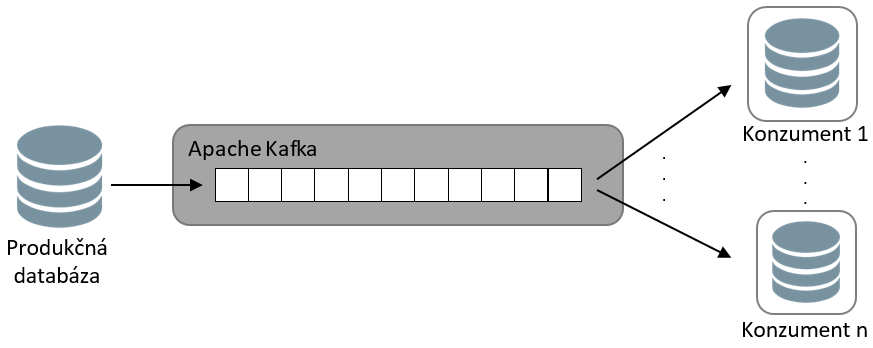
\includegraphics[width=15cm]{figures/CDC_1.PNG}
\caption{Koncept distribúcie zmenených dát}
\label{fig:CDC}
\end{center}
\end{figure}

\subsection{Dátové sklady}
% http://enos.itcollege.ee/~gseier/C__DOCUME~1_GUSTAV_LOCALS~1_TEMP_plugtmp_Attunity_CDC_White_Paper.pdf
V dátových skladoch sa uchovávajú dáta a ich história z viacerých databáz za účelom analytických výpočtov. Aktuálne najpoužívanejším riešením na napĺňanie dátových skladov je ETL\footnote{Export, transform, load}. Tento proces funguje v zmysle periodického nahrávania veľkého množstva dát do dátových skladov. Tento proces sebou ale nesie nevýhody, ktoré v minulosti neboli tak podstatné, no v dnešnej dobe už sú. Použitím CDC miesto ETL je možné niektoré z týchto nevýhod obmedziť. Dátové sklady sa za pomoci CDC napĺňajú priebežne a nie periodicky, takže dáta nad ktorými sa vykonáva analýza budú skoro vždy aktuálne. Nakoľko sa každá zmena zapisuje jednotlivo a nie pomocou veľkého balíčku, neobmedzí to beh systémov, zamedzí nutnosti systémových prestojov a zároveň to redukuje cenu za túto operáciu. Premiestnením iba zmenených údajov CDC vyžaduje oveľa menej zdrojov na presun a transformáciu dát. To zníži náklady na hardvér, softvér a aj ľudské zdroje. \cite{attunity:etl_cdc}

\subsection{Replikácia dát}
Jedným z využití CDC je replikácia dát do iných databáz napríklad v zmysle vytvorenia zálohy dát, ale taktiež je možné CDC využiť pri implementácií zaujímavých analytických požiadavkov. Predstavme si, že máme produkčnú databázu a špecializovaný analytický systém na ktorom chceme spustiť analýzu. V tomto prípade je nutné dostať dáta z produkčnej databáze do analytického systému a CDC je možnosť, ktorá nám to umožní. Ďalším využitím môže byť prísun dát ostatným tímom, ktoré na základe nich môžu napríklad vypočítavať a smerovať svoju marketingovú kampaň, napríklad na užívateľov, ktorí si objednali istý konkrétny produkt. Nakoľko nechceme aby sa takýto výpočet vykonával nad produkčnou databázou ale skôr nad nejakou separovanou databázou, tak opäť je možné využiť CDC na propagáciu dát do separovanej databáze, kde si už marketingový tým môže vykonávať akokoľvek náročné výpočty.

\subsection{Microservice Architecture}
Ďalšie využitie CDC je vhodné pri použití Microservice architecture, kde je doména rozdelená na niekoľko služieb, ktoré potrebujú medzi sebou interagovať. Pre príklad máme tri mikro služby: objednávaciu aplikáciu na spracovávanie užívateľských objednávok, produktovú službu, ktorá sa stará o produktový katalóg, a nakoniec máme skladovú službu, ktorá kontroluje reálne množstvo produktových vecí na sklade. Je zreteľné, že na správne fungovanie bude objednávacia aplikácia vyžadovať dáta od produktovej a skladovej služby. Jednou z možností je, že objednávacia aplikácia bude priamo komunikovať s ostatnými službami napríklad pomocou REST API\footnote{\url{https://cs.wikipedia.org/wiki/Representational_State_Transfer}}, čím ale bude úzko spojená a závislá na chode danej služby. Ak by takáto služba zlyhala/spadla tak nebude fungovať celá aplikácia. Druhou možnosťou je práve využiť CDC, ktoré odzrkadľuje použitie Event Sourcing paternu\footnote{\url{http://microservices.io/patterns/data/event-sourcing.html}}. Produktová a skladová služba budú poskytovať sled zmenených dát a objednávacia aplikácia ich bude zachytávať a udržiavať kópiu časti týchto dát, ktoré ju zaujímajú, vo vlastnej lokálnej databáze. Ak by v takomto prípade niektorá zo služieb zlyhala, tak objednávacia aplikácia môže naďalej fungovať.

\subsection{Ostatné}
Bežnou praxou vo väčších aplikáciách je používanie cache pre rýchly prístup k dátam na základe špecifických dotazov. V takýchto prípadoch je potrebné riešiť problémy updatu cache alebo jej zmazania, pokiaľ sa isté dáta zmenia.

Riešenie fulltextového vyhľadávania pomocou databáze nie je veľmi vhodné a namiesto toho sa používa SOLR\footnote{\url{http://lucene.apache.org/solr/}} alebo Elasticsearch\footnote{\url{https://www.elastic.co/}}, čo sú systémy, ktoré potrebujú byť synchronizované z dátami v primárnej databáze. 


\section{Odchytávanie zmien v databáze}
Každý databázový systém (\nom{DBMS}{Database management system}) má svoj log súbor, ktorý používa na zotavenie sa po páde a odvolaní transakcií, ktoré ešte neboli potvrdené, alebo na replikáciu dát voči sekundárnym databázam alebo inej funkcionalite. Či už to sú transakčné, binárne alebo replikačné logy, vždy v sebe udržujú všetky transakcie, ktoré boli úspešne vykonané nad databázou, a preto sú vhodné na odchytávanie zmien v databázach pre projekt Debezium. Konkrétne v MySQL databáze sa volá \textbf{binlog} (\ref{mysql:binlog}). Nakoľko sú tieto logy plne transparentné voči aplikácii, ktorá do databáze zapisuje, výkon aplikácie nebude nijako ovplyvnený čítaním týchto logov.

\subsection{Apache Kafka}
Apache Kafka je open-source distribuovateľná platforma na streamovanie správ vyvinutá firmou Apache Software Foundation. Umožňuje vytvárať a sledovať tok záznamov podobný fronte správ. Tento tok ukladá spôsobom odolným voči chybám. Hlavným použitím Kafky je vytváranie dátových potrubí v reálnom čase, ktoré spoľahlivo získavajú dáta medzi systémami alebo aplikáciami a budovanie aplikácií na streamovanie v reálnom čase, ktoré transformujú alebo reagujú na prúdy dát. Kafku je možné spustiť ako cluster na jednom, alebo viacerých serveroch, ktoré ukladajú toky záznamov v kategóriách nazvaných \textbf{topiky}. Každá správa v Kafke pozostáva z kľúča, hodnoty a časovej značky. Každej správe Kafka priradí sekvenčné identifikačné číslo nazývané \textbf{offset}, ktoré unikátne identifikuje každý záznam a jeho poradie v topiku.

Kafka pozostáva zo štyroch základný API:\cite{Kafka}
\begin{itemize}
\item \textbf{Producer API}, ktoré umožňuje aplikáciám publikovať sled záznamov do jedného alebo viacerých topikov.
\item \textbf{Consumer API}, ktoré umožňuje konzumovať existujúce topiky a spracovať sled záznamov, ktorý obsahujú.
\item \textbf{Streams API}, ktoré umožňuje aplikáciám chovať sa ako spracovávateľ sledu záznamov. Aplikácie pohlcujú prichádzajúci sled a produkujú transformovaný výstupný sled.
\item \textbf{Connector API}, ktorý umožňuje vytvárať znovu použiteľné dátové spojenia na publikovanie a konzumovanie záznamov, ktoré pripoja topiky k existujúcim aplikáciám alebo dátovým systémom.
\end{itemize}

\begin{figure}[H]
\begin{center}
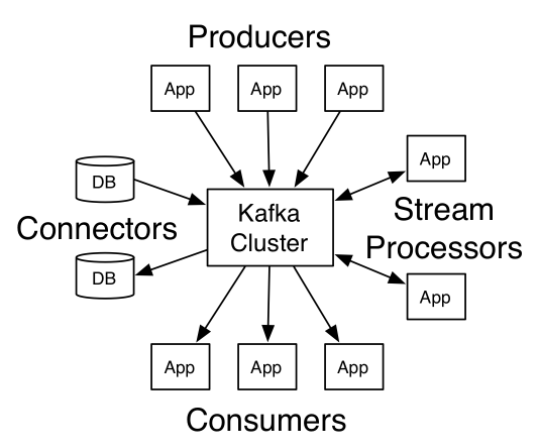
\includegraphics[width=9cm]{figures/kafka_hierarchy.PNG}
\caption{Hierarchia Apache Kafka}
\label{fig:kafka_hierarchy}
\end{center}
\end{figure}

Projekt Debezium využíva posledné zmienené \textit{Connector API} použitím Kafka Connect frameworku (\ref{kafka_connect}), pomocou ktorého implementuje CDC pre jednotlivé databázové systémy.

\subsection{Infraštruktúra správ pomocou Apache Kafka}
Apache Kafka poskytuje sémantické pravidlá, ktoré dobre vyhovujú potrebám projektu Debezium. Prvým z nich je, že všetky správy v Kafke majú kľúč a hodnotu. Táto vlastnosť sa využíva na zjednotenie správ, ktoré spolu súvisia a to konkrétne tak, že na základe primárneho kľúča v tabuľke, ktorej zmena sa zmena týka je možné štruktúrovať kľúč správy a hodnota správy bude reprezentovať konkrétnu zmenu.

Kafka taktiež garantuje poradie správ metódou FIFO\footnote{First in First out}, čím sa zabezpečí správne poradie zmien, ktoré bude konzument prijímať. Táto vlastnosť je veľmi dôležitá, nakoľko ak by nastala situácia \textit{insert} a následne \textit{update} alebo dve \textit{update} akcie za sebou, tak musí byť zabezpečené, aby sa ku konzumentovi dostali v správnom poradí inač by mohla nastať nekonzistencia voči dátam v primárnej databáze a dátam, ktoré si udržiava konzument.

Kafka je pull-based systém, čo znamená, že konzument je sám sebe pánom a drží si informáciu o tom, ktoré správy z konkrétneho topiku už prečítal resp. kde chce začať čítanie ďalších správ. Takto môže sledovať aktuálne pribúdajúce správy, ale taktiež sa môže zaujímať aj o správy z minulosti.

Zmien v databázach môže byť veľmi veľa, čo spôsobí veľké množstvo udalostí, a preto je nutné spomenúť ďalšiu výhodu Kafky a to jej škálovateľnosť. Kafka podporuje horizontálnu škálovateľnosť a jednotlivé topiky môžu byť rozdelené na viacero partícií. Je ale nutné si uvedomiť, že poradie zmien je garantované iba na konkrétnej partícii. Kafka zabezpečí, že všetky správy s rovnakým kľúčom budú na rovnakej partícii, čím sa garantuje ich správne poradie, ale môže nastať situácia, že udalosť s iným kľúčom, ktorá reálne nastala neskôr, môže byt konzumentom spracovávaná skôr, čo môže, ale aj nemusí vadiť v závislosti na konkrétnej funkcionalite konzumenta.

\subsection{Kafka Connect}\label{kafka_connect}
Kafka Connect je framework, ktorý umožňuje jednoduchú implementáciu dátových spojení (konektorov) s Kafkou. Tieto konektory majú na starosti dáta, ktoré vstupujú alebo vystupujú z Kafky. Nazývajú sa \textit{source}(vstupujúce dáta resp. import) konektory alebo \textit{sink}(vystupujúce dáta resp. export) konektory. Debeziové konektory majú na starosti naplňovanie Kafky, takže sa používa \textit{source} konektor. Kafka Connect ponúka možnosť na riešenie offsetu. Na rozdiel od Kafka offsetu, ktorý je priradený každej správe v topiku, Kafka Connect offset si udržuje informáciu o pozícií poslednom prečítanom evente z binlogu. Môže nastať situácia, že konektor zhavaruje a bude musieť byť reštartovaný. V takomto prípade konektor potrebuje vedieť ako ďaleko v čítaní logu bol a kde má s čítaním pokračovať. 

\begin{figure}[H]
\begin{center}
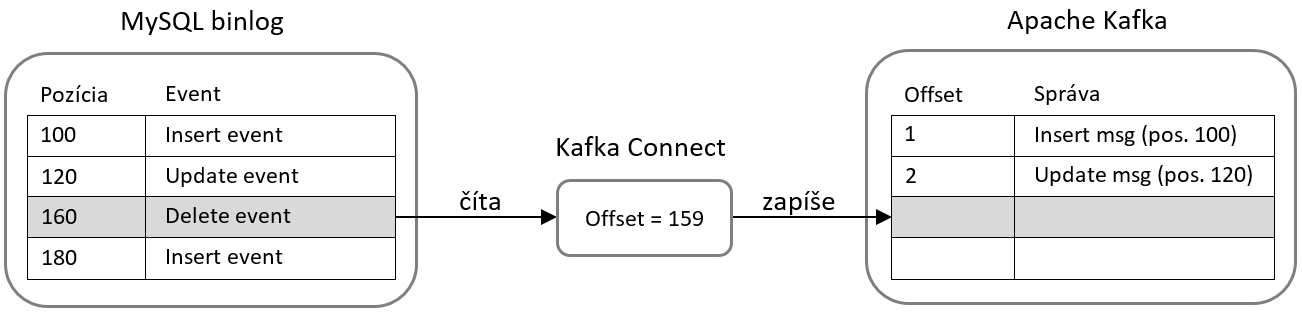
\includegraphics[width=15cm]{figures/kafka_offsets.PNG}
\caption{Príklad nastavenia Kafka a Kafka Connect offsetov}
\label{fig:kafka_offsets}
\end{center}
\end{figure}

Pre príklad si povedzme, že jedna udalosť v MySQL binlogu má veľkosť 20. Na obrázku \ref{fig:kafka_offsets} je možné vidieť situáciu, kedy sa konektoru podarilo prečítať a spracovať udalosti z MySQL binlogu nachádzajúce sa na pozíciách 100 a 120. Ich príslušné správy sú dostupné v Kafke s nastaveným Kafka offsetom 1 a 2. Kafka Connect má v tejto situácií offset rovný 159, nakoľko to je posledná prečítaná pozícia. Použitím Kafka Connect je zabezpečené, že po každom spracovaní udalosti konektor potvrdí svoj offset, a ak by konektor musel byť reštartovaný, tak môže zistiť posledný potvrdený offset a pokračovať v čítaní logu z nasledujúcej pozície.

Ďalším prínosom je možnosť konfigurácie schémy správ. Kafka Connect má svoj systém na definovanie typu dát, ktorým umožňuje popísať štruktúru kľúčov a hodnôt v správach. Bližšie popísané v kapitole \ref{ssec:message_structure}.

Kafka Connect je clustrovateľná, takže je možné v závislosti na špecifikácií rozdeliť konektor a jeho úlohy medzi viacero uzlov. Taktiež ponúka bohatý eko-systém konektorov. Na stránkach Confluent\footnote{\url{https://www.confluent.io/product/connectors/}} je možné si stiahnuť rôzne typy či už \textit{sink} alebo \textit{source} konektorov.
Príklad CDC topológie s použitím Kafka Connect je na obrázku \ref{fig:CDC_topology} \cite{debezium:devoxx}. Zámerom v danom obrázku je zdieľať dáta dvoch tabuliek z MySQL databáze a jednej tabuľky z Postgres databáze. Každá monitorovaná tabuľka je vyjadrená jedným topikom v Kafke. Prvým krokom je nastavenie clusterov v Apache Kafka, pričom je to možné spustiť na jednom alebo viacerých clusteroch. Ďalším krokom je nastavenie Kafka Connect, ktorá je oddelená od Apache Kafka a beží v separátnych procesoch alebo clustroch, a ktorá bude spravovať spojenie z Apache Kafka. Následne je nutné nasadiť inštancie Debezium konektorov do Kafka Connect a to konkrétne MySQL a Postgres konektory, nakoľko sú sledované dáta v týchto DBMS. Posledným krokom je konfigurácia aspoň jedného \textit{sink} konektoru, ktorý bude spracovávať dané topiky v Apache Kafka a odosielať ich inému systému (konzumentovi). Na konkrétnom príklade je použitý Elasticsearch konektor nakoľko je konzumentom Elasticsearch.

\begin{figure}[H]
\begin{center}
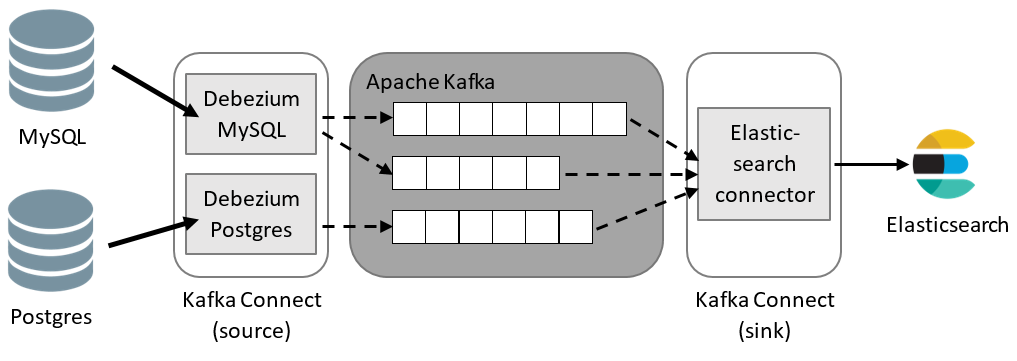
\includegraphics[width=15cm]{figures/CDC_topology.PNG}
\caption{CDC topológia z Kafka Connect}
\label{fig:CDC_topology}
\end{center}
\end{figure}

\subsection{Štruktúra správy} \label{ssec:message_structure}
Ako už bolo spomenuté, správy v Kafke obsahujú kľúč, v prípade Debezia je to primárny kľúč v tabuľke, a hodnotu, ktorá má komplexnejšiu štruktúru skladajúcu sa z:
\begin{itemize}
\item \textbf{before} stavu, ktorý v sebe nesie predchádzajúci stav data, ktoré sa mení. V prípade, že nastane \textit{insert} event, táto hodnota bude prázdna, nakoľko práve vzniká a nemá žiadny predchádzajúci stav.
\item \textbf{after} stavu, ktorý v sebe nesie nový stav dát. Táto hodnota môže byť opäť prázdna a to v prípade \textit{delete} udalosti.
\item \textbf{source} informácie, ktoré  obsahujú metadáta o pôvode danej zmeny. Tieto dáta sú závislé na type databáze, ktorá sa sleduje. Pre MySQL databázu sa napríklad skladá z informácií ako meno databázového serveru, názvu a pozície logovacieho súboru, z ktorého číta, názvu databáze a tabuľky, timestamp a pod.
\end{itemize}

Kafka dokáže spracovávať akýkoľvek druh textových a binárnych dát, takže jej na tejto logickej štruktúre nezáleží. Na odosielanie správ sa používajú konvertory, ktoré prevádzajú správu do formy v ktorej bude odosielaná. Použitie Kafka Connect prináša možnosť využiť dostupné konventory, ktoré pokytuje. Pre Debezium to sú:

\begin{itemize}
\item \textbf{JSON}, do ktorého je možnosť zahrnúť informácie o schéme dát, na základe ktorej môžu konzumenti správne interpretovať prijatú správu. Tento formát je výhodné používať počas vývoja aplikácie nakoľko je čitateľný pre človeka. Ukážku správy vo formáte JSON je možné zhliadnuť v prílohe \ref{code:schemaExample}.
\item \textbf{Avro}, ktorý má veľmi efektívnu a kompaktnú reprezentáciu vhodnú na produkčné účely. Takáto správa nie je vo forme, aby ju človek bez úprav mohol prečítať, nakoľko je to binárna reprezentácia správy. V týchto správach sa nenachádza informácia o schéme tabuľky, ale iba identifikátor na danú schému a jej verziu, ktorú je možné získať pomocou registru schémat, čo je ďalšia časť ekosystému Kafky. Konzument môže získať konkrétnu schému z registrov a na základe nej interpretovať binárne dáta, ktoré dostal.
\end{itemize}

% \subsection{Inicializácia}
    \chapter{Aktuálne riešenie MySQL konektoru}
Projekt Debezium sa zkladá z viacerých častí. Hlavnou časťou je modul systému, ktorý je spoločný pre všetky typy konektorov podporovaných Debeziom. Tento modul zaobstaráva základnú funkcionalitu spojenú s CDC, ktorú tento systém podporuje. Definuje model sledovaných dát, na základe ktorých si systém udržuje aktuálne schémata tabuliek a ich dátový stav v pamäti. Jedným z týchto podporovaných konektorov je aj konektor pre MySQL databázu \ref{debezium:mysql_connector}.

\textbf{TODO co viac k tomu ?} 

\section{MySQL konektor}\label{debezium:mysql_connector}
Minimálnou podporovanou verziou MySQL je aktálne verzia 5.6. MySQL konektor Debezia dokáže sledovať zmeny v databázy na úrovni jednotlivých riadkov v tabuľkách pomocou čítania databázového binlogu (\ref{mysql:binlog}). Pri prvom pripojení na MySQL server si konetor vytvorí aktuálny obraz všekých tabuliek (\ref{debezium:conistent_snapshot}) a následne sleduje všetky komitnuté zmeny, na základe ktorých vytvára jednotlivé \textit{insert}, \textit{update} a \textit{delete} eventy. Pre každú tabuľku je vytvorený separátny topik v Kafke v ktorom sa ukladajú eventy spojené z danou tabuľkou. Týmto spôsobom je zabezpečený štart s konzistentným obrazom všetkých dát.

Konektor je taktiež veľmi tolerantný vočí chybám. Zároveň s čítaním událostí z binlogu si konektor ukladá ich pozíciu. Ak by nastala akákolvek situácia pri ktorej by konektor prestal pracovať a bol by nutný jeho reštart, tak jednoducho začne čítanie binlogu na pozícii na ktorej skončil pred pádom. Konektor sa bude rovnko správať aj keby chyba a jeho pád nastali počas prvotného vytvárania aktuálneho obrazu.

\subsection{Binárny log} \label{mysql:binlog}
v MySQL je možné implementovať CDC na základe sledovania binárneho logu v skratke nazývaného binlog\cite{mysql:reference_manual}. Binlog obsahuje všetky události, ktoré popisujú zmeny vykonané nad MySQL databázou ako napríklad vytváranie tabuliek alebo zmena dát. Poradie týchto události je zachované voči reálnemu poradiu ako boli SQL dotazy vykonávané. Toto binárne logovanie sa využíva na dva základne účely:
\begin{itemize}
\item Pre \textbf{replikáciu}, kde binlog na master replikačnom serveri sprostredkuváva záznamy o zmenách, ktoré majú byť odoslané slave serverom. Master server odošle události nachádzajúce sa v binlogu slave serveri, ktorý tieto události vykoná u seba za účelom udržania rovnakého dátového stavu ako je na master replikačnom serveri.
\item Pre \textbf{obnovu systému z chybového stavu} anlicky nazývanú \textbf{recovery}. Po  nahraní zálohy databáze sú znovu spustené události zaznamenané v binlogu, ktoré nastali po vytvorení zálohy, čím sa zabezpečí konzistentný stav databázových dát z dátami v dobe zlyhania databázového serveri.
\end{itemize}

Binárny log neobsahuje události, ktoré nemajú žiadny efekt na dáta ako napríklad  SELECT alebo SHOW. Události môžu byť do logu zapisované v rôznych formátoch, na základe ktorých sa mení aj spôsob replikácie dát. Tieto formáty logovania sú:
\begin{itemize}
\item \textbf{Statement-based} logovanie, v ktorom události obsahujú SQL dotazy, ktoré produkujú zmeny v dátach (INSERT, UPDATE, DELETE). V rámci tohto logovanie môže taktiež obsahovať dotazy, ktoré môžu iba potencionálne meniť dáta napríklad DELETE dotaz, ktorý sa nespáruje so žiadnymi dátami. Pri replikácií slave server číta binlog a zaradom vykonáva SQL dotazy, ktoré obsahujú jednotlivé události.
\item \textbf{Row-based} logovanie, v ktorom události popisujú zmeny pre jednotlivé riadky v tabuľkách. Pri replikácií sa kopírujú události, ktoré reprezentujú zmeny riadkov v tabuľkách na slave serveri. 
\end{itemize}

Pre účely CDC v Debeziu je používané row-based logovanie, nakoľko zalogované události obsahujú zmeny pre konkrétne riadky v tabuľkách a tým pádom nieje nutné dopočítavať dáta, ktoré by boli na základe daného dotazu zmenené. Master server ukladá do binlogu iba kompletné a vykonané transakcie, čo znamená, že sa tam nemôžu objaviť syntakticky nevalidné dotazy. V MySQL konektoru teda nie je nutné sledovať korektnosť parsovaných dotazov.

Pomocou SQL dotazu \textit{SHOW BINARY LOGS} je možné vylistovať aktuálne existujúce binárne logy na serveri. Následne dotazom \textit{SHOW BINLOG EVENTS [IN 'log\_name']  [FROM pos] [LIMIT [offset,] row\_count]} je možné sledovať informácie o všetkých událostiach obsiahnutých v danom binlogu ako sú napríklad typ události, jeho začiatočná a jeho konečná pozícia v logu. Na čítanie a spracovávanie binlogu ponúka MySQL nástroj \textit{mysqlbinlog}, ktorý je možné spustiť príkazom \textit{mysqlbinlog [options] log\_file}. Prvý riadok události vždy obsahuje prefix \textit{\# at} za ktorým následuje číslo reprezentujúce pozíciu události v binlogu. Podľa základného nastavenia MySQL zobrazuje mysqlbinlog události týkajúce sa zmien na úrovní riadkov zakódované ako base-64\footnote{Typ kódovania, ktorý prevádza binárne dáta na postupnost znakov} použitím interného príkazu \textit{BINLOG}. Aby bolo možné vidieť tento pseudokód je možné použiť prepínač \textit{---verbose} alebo \textit{-v}. Na výstupe bude možné vidiet tento pseudokód na riadkoch, ktoré budú začínať prefixom  \textit{\#\#\#}. Použitím prepínača \textit{---verbose} alebo \textit{-v} dvakrát, môžeme nastaviť aj zobrazovanie dátových typov a iných metadát pre každý stĺpec. Aby sa v logu nezobrazoval interný príkaz \textit{BINLOG} a zakódovaná hodnota události, je možné použiť prepínač \textit{---base64-output=DECODE-ROWS}. Kombináciou týchto prepínačov získame možnosť pohodlne sledovat obsah události týkajúcich sa zmien v dátach. \cite{mysql:reference_manual}
% https://dev.mysql.com/doc/refman/5.7/en/mysqlbinlog-row-events.html

Pre Debezium sú dôležité události typu:
\begin{itemize}
\item \textbf{Query}, v ktorom sa objavujú dotazy na zmenu štruktúry databáze (\nom{DDL}{Data definition language}) ako je možné vidiet na poslednom riadku príkladu události \ref{code:binlog_query_ddl}.
\item \textbf{Table\_map}, pomocou ktorého binlog mapuje konkrétne tabuľky na identifikátor, ktorým sa následne tieto tabuľky referencuje. Príklad tejto události je možné vidieť v príklade \ref{code:binlog_update_row} na pozícii 552 a jeho následné použitie pre událosť na pozícii 621. 
\item \textbf{Update\_rows}, ktorý obsahuje informácie o zmene dát na úrovni riadkov, ako je možné vidiet na události v príklade \ref{code:binlog_update_row} na pozícii 621.
\item \textbf{Write\_rows}, ktorý obsahuje infomrácie o novo vzniknutých dátach.
\item \textbf{Delete\_rows}, ktorý obsahuje informácie o zmazaných dátach.
\end{itemize}

\lstinputlisting[language=bash,
			caption=Query událost z binárneho logu MySQL, 
            label=code:binlog_query_ddl]
            {code/3/binlog_query_ddl}

\lstinputlisting[language=bash,
			caption=Table\_map a Update\_rows události z binárneho logu MySQL, 
            label=code:binlog_update_row]
            {code/3/binlog_update_row}
            
\subsection{Aktuálny obraz tabuliek} \label{debezium:conistent_snapshot}
% http://debezium.io/docs/connectors/mysql/#snapshot
Po nakonfigurovaní a prvom spustení MySQL konektoru sa podľa základného nastavenia spustí tvorba aktuálneho obrazu tabuliek sledovanej databáze. Vo väčšine prípadoch už MySQL binlog neobsahuje kompletnú historóriu databáze a preto je tento mód v základnom nastavení. 

Pri kažnom vytváraní aktuálneho obrazu, konektor postupuje podľa týchto krokov\cite{debezium:consistent_snapshot}:
\begin{enumerate}
\item Aktivuje globálny zámok čítania (read lock) aby zabránil ostatným databázovým klientom v zapisovaní.
\item Spustí transakciu s izoláciou na opakované čítanie (repeatable read)\footnote{Stupeň izolácie založený na používaní \textit{read} a \textit{write} zámkoch, ktorý ale nezabráni prítomnosti fantómov vznikajúcich v stiuácii, keď v jednej transakcii podľa rovnakého dotazu čítame dáta 2x z rôznymi výsledkami, pretože v medzičase stihla iná transakcia vytvoriť alebo zmazať časť týchto dát.}, aby všetky nasledujúce čítania v rámci tejto transakcie boli voči jednému konzistentnému obrazu.
\item Prečíta aktuálnu pozíciu binlogu.
\item Prečíta schéma databází a tabuliek na základe konfigurácie konektoru.
\item Uvolní globálny zámok, aby ostaný databázový klienti mohli znovu zapisovať do databáze.
\item Voliteľne zapíše zmeny DDL do Kafka topiku vrátane všetkých potrebných SQL dotazov.
\item Oskenuje všetky databázové tabuľky a vygeneruje príslušné \textit{create} události  Kafka topiky pre jednotlivé riadky v tabuľkách.
\item Commitne transakciu.
\item Do konektorového offsetu zaznamená, že úspešne ukončil vytváranie obrazu.
\end{enumerate}

Transakcia vytvorená v druhom kroku nezabráni ostatným klientom upravovať dáta, ale poskytne konektoru konzistentný a nemenný pohľad na dáta v tabuľkách. Nakoľko transakcia nezabráni klientom aplikovať DDL zmeny, ktoré by mohli vadiť konektoru pri čítaní pozície a schémat v binlogu, je nutné v prvom kroku použiť globálny zámok na čítanie k zamedzeniu tohto problému. Tento zámok je udžiavaný na veľmi krátku dobu potrebnú pre konektor na vykonanie krokov tri a štyri. V piatom kroku je tento zámok uvolnený predtým, než konektor vykoná väčšinu práce pri kopírovaní údajov.

\textbf{Note: moze byt popisane este viac ak by bolo potrebne nahrabat strany :)}

%  DDL PARSER 
% http://debezium.io/blog/2016/04/15/parsing-ddl/
\section{DDL parser}
Pri čítaní binárneho logu MySQL konektor parsuje DDL dotazy na základe ktorých si v pamäti vytvára modely schémat každej tabuľky podľa toho ako sa vyvíjali v čase. Tento proces je veľmi dôležitý, pretože konekor generuje události pre tabuľky, v ktorých definuje schéma tabuľky v čase, kedy daná událosť vznikla. Aktálne schéma sa nemôže použiť, nakoľko sa môže zmeniť v danom čase pípadne na danej pozícii v logu na ktorej konektor číta. 

Konektor produkuje správy použitím Kafka Connect Schemas, ktoré definujú jednoduchú dátovú štruktúru obsahujúcu názvy a typy polí a spôsob organizácie týchto polí. Pri generovaní správy na událosť týkajúci sa dátovej zmeny je najprv nutné mať Kafka Connect \inlinecode{Schema} objekt, v ktorom definujeme všetky potrebné polia. Následne je nutné konvertovať usporiadané pole hodnôt stĺpcov do Kafka Connect \inlinecode{Struct} objektu na základe polí a ich hodnôt z odchytenej události.

Ak Debezium konektor odchytí DDL událost, stačí mu aktualizovať model, ktorý si drží v pamäti a ten následne použiť na generovanie \inlinecode{Schema} objektu. V rovnakom čase sa vytvrí komponenta, ktorá bude používať tento \inlinecode{Schema} objekt na vytváranie \inlinecode{Struct} objektu z hodnôt v odchytenej události. Tento proces sa vykoná raz a použije sa na všetky DML údálosti až do doby pokiaľ sa neodchytí ďalší DDL dotaz, po ktorom bude opäť nutné aktualizovať model v pamäti.

Nato aby bolo možné túto akciu vykonať je nutné parsovať DDL dotazy, pričom pre potreby Debezia stačí vedieť rozpozať iba malú časť z celej DDL gramatiky. Model, ktorý sa udržiava v pamäti a zbytok funkcionality spojený z generovaním \inlinecode{Schema} objektu a konventoru hodnôt na \inlinecode{Struct} objekt je generické nakoľko nie je priamo spojené z MySQL.

\subsection{Framework na parsovanie DDL}
Keďže Debezium nenašlo žiadnu použiteľnú knižnicu na parsovanie DDL, rozhodlo sa implementovať vlastný framework podľa ich potrieb, ktoré sú\cite{debezium:parse_ddl}:
\begin{itemize}
\item Parovanie DDL dotazov a aktualizácia modelu v pamäti.
\item Zameranie sa na podstatné dotazy ako sú \inlinecode{CREATE}, \inlinecode{UPDATE} a \inlinecode{DROP} tabuliek, pričom sa ostané dotazy budú ignorovať bez nutnosti ich parsovať.
\item Štruktúra kódu parsru, ktorá bude podobná dokumentácii MySQL DDL gramatiky a názvoslovie metód, ktorá bude odzrkadľovať pravidlá gramatiky. Takúto implementáciu je jednoduhšie udržiavať v priebehu času.
\item Umožniť vytvorenie parserov pre PostreSQL, Oracle, SQLServer a všetkých ostatných DBMS, ktoré budú potrebné.
\item Umožniť prispôsobenie pomocou dedičnosti a polymorfismu.
\item Uľahčit vývoj, ladenie a testovanie parserov.
\end{itemize}

Výsledný framework pozostáva z tokenizeru, ktorý konvertuje DDL dotaz v jednom reťazci na sekvenciu tokenov. Každý token reprezentuje interpunkčné znamienka, citované reťazce, slová a symboly, kľučové slová, komentáre a ukončujúce znaky ako napríklad bodkočiarku pre MySQL. DDL parser prechádza sled tokenov a volá metódy na spracovanie variácii sady tokenov.Parser taktiez využíva interny \inlinecode{DataTypeParser} na spracovanie dátových typov SQL, ktoré si je možné pre jednotlivé DBMS ručne zaregistrovať.

\inlinecode{MySqlDdlParser} trieda dedí od základnej triedy \inlinecode{DdlParser} a sprostredkuváva celú parsovaciu logiku špecifickú pre MySQL. Napríklad DDL dotaz \ref{code:ddl_sql_example} je možné sparsovať podľa ukážky \ref{code:mysql_ddl_parse_example_old}.

\lstinputlisting[language=MySQL,
			caption=DDL dotaz v MySQL, 
            label=code:ddl_sql_example]
            {code/3/ddl_example.sql}
            
\lstinputlisting[language=Java2,
			caption=Parsovanie dotazu pomocou MySqlDdlParseru, 
            label=code:mysql_ddl_parse_example_old]
            {code/3/mysql_ddl_parse_example_old.java}
            
\inlinecode{Tables} objekt reprezentuje model uložený v pamäti konkrétnej databáze. Parser zprocesuje jednotlivé DDL dotazy a aplikuje ich na odpovedajúce definície tabuliek nachádzajúce sa v \inlinecode{Tables} objekte.

\subsection{Implementácia MySQL DDL parsru}
Každá implementácia \inlinecode{DdlParser} implementuje metódu, ktorá parsuje DDL dotazy poskytnuté v reťazci. Táto metóda vytvára nový \inlinecode{TokenStream} pomocou \inlinecode{DdlTokenizer}, ktorý rozdelí znaky v reťazci do typovaných \inlinecode{Token} objektov. Následne volá ďalšiu parsovaciu metódu v ktorej nastaví lokálne premenné a snaží sa zaradom parsovať DDL dotazy do doby, kým žíadny ďalší nenájde. Ak by počas parsovania nastala chyba napríklad že by sa nenašla zhoda, parser vygeneruje \inlinecode{ParsingException}, ktorá obsahuje riadok, stĺpec a chybovú správu oznamujúcu aký token bol očakávaný a aký sa našiel. V prípade chyby sa \inlinecode{TokenStream} pretočí na začiatok, aby sa prípadne mohla použiť implementácie iného parseru.

Pri každom volaní metódy \inlinecode{parseNextStatement} je predavaný objekt \inlinecode{Marker}, ktorý ukazuje na začiatočnú pozíciu parsovaného dotazu. Vďaka polymorfizmu \inlinecode{MySqlDdlParser} prepisuje implementáciu \inlinecode{parseNextStatement} metódy (ukážka \ref{code:mysqlParseNextStatement}), v ktorej kontroluje, čí prvý token vyhovuje niektorému z typov MySQL DDL gramatiky. Po najdení vyhovujúceho tokenu sa zavolá odpovedajúca metóda na ďalšie parsovanie. 

Pre príklad, ak by parser chcel parsovať dotaz začínajúci na \textit{CREATE TABLE ...}. Prvým parsované slovo je \textit{CREATE}, čím by sa podľa ukážky z kódu \ref{code:mysqlParseNextStatement} zavolá metóda \inlinecode{parseCreate}. V nej sa toto slovo skonzumuje a rovnakým spôsobom nastáva kontrola druhého slova, kde sa po vyhodnotení hodnoty \textit{TABLE} zavolá metóda \inlinecode{parseCreateTable} (ukážka \ref{code:parseCreateTable}). Táto metóda odzrkadľuje následovné pravidlá MySQL gramatiky pre \mbox{\textit{CREATE TABLE}}:
\newline
\begin{lstlisting}[language=MySQL, frame=none, numbers=none]
CREATE [TEMPORARY] TABLE [IF NOT EXISTS] tbl_name
    (create_definition,...)
    [table_options]
    [partition_options]

CREATE [TEMPORARY] TABLE [IF NOT EXISTS] tbl_name
    [(create_definition,...)]
    [table_options]
    [partition_options]
    select_statement

CREATE [TEMPORARY] TABLE [IF NOT EXISTS] tbl_name
    { LIKE old_tbl_name | (LIKE old_tbl_name) }

create_definition:
    ...
\end{lstlisting}

Metóda \inlinecode{parseCreateTable} sa snaží najprv skonzumovať nepovinné slovo \textit{TEMPORARY}, potom slovo \textit{TABLE}, nepovinný fragment \textit{IF NOT EXISTS} a následne konzumuje a parsuje názov tabuľky. Ak by dotaz obsahoval fragment \textit{LIKE otherTable}, tak sa použije objekt \inlinecode{Tables}, z ktorého sa získa definícia odkazovanej tabuľky. V ostatných prípadoch sa na úpravu stávajúcej tabuľky použije \inlinecode{TableEditor} objekt. Takýmto spôsobom parser pokračuje vo svojej činnositi ďalej a snaží sa parsovať dotaz na základe pravidiel gramatiky.

\textbf{TODO: spisat info ohladne ukladanych informacii}
    \chapter{Syntaktická analýza}
Syntaktickou analýzou (slangovo z angličtiny tiež \textbf{parsovaním}) sa v teórii rozumie konštrukcia derivačného stromu vety bezkontextového jazyka\cite{CVUT:program_language} popísaného v kapitole \ref{CFG}. Program, ktorý vykonáva túto úlohu sa volá syntaktický analyzátor (slangovo \textbf{parser}). Počas konštrukcie derivačného stromu parser zachováva hierarchické usporiadanie symbolov, ktoré je vhodné pre ďalšie spracovanie.

Parsovanie je taktiež možné si predstaviť ako inverziu k napĺňaniu šablón. Šablóna definuje napríklad štruktúru textu s variabilnými premennými, ktoré je potrebné naplniť dátami a parsovanie identifikuje túto šablónu a extrahuje dáta, ktoré boli do nej vložené.

\begin{figure}[H]
\begin{center}
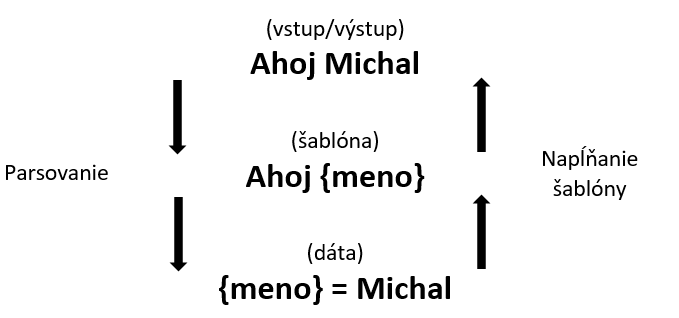
\includegraphics[width=10cm]{figures/templatingAndParsing.PNG}
\caption{Príklad parsovania a napĺňania šablóny}
\label{fig:templatingAndParsing}
\end{center}
\end{figure}

Podstata parsovania je veľmi dôležitá, pretože rôzne entity potrebujú dáta na spracovanie v rôznych formátoch. Parsovanie umožňuje transformovať získané dáta tak, aby im mohol porozumieť špecifický software. 

\section{Teória parsovania}
Na správne pochopenie problému parsovania je nutné najprv zadefinovať základné pojmy, ktoré sú s ním spojené. Teória parsovania je postavená na teórii jazykov, gramatík a automatov, z ktorej najdôležitejšie pojmy sú definované v rámci tejto sekcie.

\subsection{Deterministický konečný automat}\label{DFA}
Konečné automaty sa používajú v rôznych oboroch ako napríklad pri prekladačoch, spracúvaní prirodzeného jazyka, pri návrhu hardwaru a ďalších \cite{demlova:automaty}. Predstavujú model systémov, ktoré rozpoznajú, či vstupný reťazec patrí do jazyka. Deterministický konečný automat (\nom{DFA}{Deterministic Finite Automaton}), taktiež aj \textit{akceptor}, je najpoužívanejší zo štyroch typov automatov.

\begin{definice}
\textit{Deterministický konečný automat} $M$ je pätica $M = (Q,\Sigma,\delta, q_0, F)$, kde
\begin{itemize}
\item $Q$ je konečná množina stavov
\item $\Sigma$ je konečná množina vstupných symbolov
\item $\delta$ je prechodová funkcia $\delta: Q \times \Sigma \rightarrow Q$
\item $q_0$ je počiatočný stav
\item $F \subseteq Q$ je množina koncových stavov \cite{demlova:automaty}
\end{itemize}
\end{definice}

Konečný automat je možné prehľadne znázorniť formou stavového diagramu. \textit{Stavový diagram} je orientovaný graf, v ktorom sú uzly ohodnotené stavmi automatu a hrany vstupnými symbolmi automatu. Z uzlu $q$ vedie hrana ohodnotená symbolom $a$ do uzlu $p$ vtedy, ak $\delta(q,a) = p$. Počiatočný stav sa označuje šípkou, ktorá neprichádza zo žiadneho iného stavu a uzly ohodnotené koncovými stavmi označujeme dvojitým krúžkom. Príklad takto znázorneného DFA je na obrázku \ref{fig:DFA_example}.

\begin{figure}[H]
\begin{center}
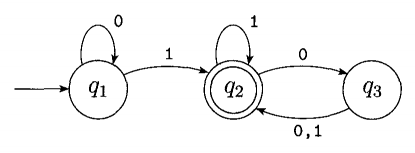
\includegraphics[width=8cm]{figures/DFA_example.PNG}
\caption{Príklad DFA znázorneného pomocou stavového diagramu}
\label{fig:DFA_example}
\end{center}
\end{figure}

\begin{definice}[\textbf{Jazyk prijímaný konečným automatom}]\label{def:regular_language}
Je daný DFA $M = (Q,\Sigma,\delta, q_0, F)$. Slovo $u \in \Sigma^*$ je \textit{prijímané} automatom $M$ práve vtedy, keď
\begin{center}
$\delta^*(q_0,u) \in F$.
\end{center}
Množina všetkých slov, ktoré automat prijíma sa nazýva \textit{jazyk prijímaný} $M$ a značíme ju $L(M)$. Platí teda
\begin{center}
$L(M) = \{\omega|\delta^*(q_0,u) \in F\}$.\cite{demlova:automaty}
\end{center}
\end{definice}

Každý jazyk $L$, pre ktorý existuje deterministický konečný automat prijímajúci tento jazyk, sa nazýva \textbf{regulárny jazyk}.

\subsection{Regulárny výraz}\label{regexp}
Regulárny výraz je ďalšia možnosť, ako popísať regulárne jazyky, ktoré sú uzatvorené vzhľadom k operáciám zjednotenia, súčinu a iterácie. Regulárne výrazy sú postavené na Kleeneho operátore(*), ktorý sa používa na označenie, že určitý prvok môže byť prítomný nula alebo nekonečne veľa krát.
\begin{definice}[\textbf{Regulárne výrazy nad abecedou}]
Je daná abeceda $\Sigma$. Množina všetkých regulárnych výrazov nad $\Sigma$ je definovaná induktívne:
\begin{itemize}
\item $\emptyset$ je regulárny výraz,
\item $\epsilon$ je regulárny výraz,
\item \textbf{a} je regulárny výraz pre každé písmeno $a \in \Sigma$,
\item pokiaľ sú \textbf{r$_1$} a \textbf{r$_2$} regulárne výrazy, tak \textbf{r$_1$ + r$_2$}, \textbf{r$_1$r$_2$} a \textbf{r$_1^*$} sú regulárne výrazy. \cite{demlova:automaty}
\end{itemize}
\end{definice}

Podpora regulárnych výrazov je dostupná u väčšiny programovacích jazykov. Pre zjednodušenie zápisu sú definované viaceré znaky, ktoré vychádzajú zo spomenutých základných operácií. Ich najčastejšie využitie je na vyhľadávanie v texte.

% You can implement a lexer using the regular expression engine provided by your language. However usually the regular expressions defined in the grammar are converted are actually converted to a finite-state machine to gain better performance.

\subsection{Bezkontextový jazyk}\label{CFG}
Bezkontextový jazyk je jazyk nad abecedou, ktorý je prijímaný bezkontextovou gramatikou (\nom{CFG}{context-free grammar}). Gramatikou sa rozumie súpis pravidiel, ktoré určujú ako vygenerovať všetky slová daného jazyka. CFG reprezentuje silnejšiu metódu popisovania jazykov, pomocou ktorej je možné opísať vlastnosti, ktoré majú rekurzívnu štruktúru.

\begin{definice}
\textit{Bezkontextová gramatika} je usporiadaná štvorica $\mathcal{G} = (N, \Sigma , S, P)$, kde
\begin{itemize}
\item $N$ je konečná množina tzv. \textit{neterminálov}\footnote{Premenné symboly, ktoré sa reprezentjú pomocou velkých písmen}
\item $\Sigma$ je konečná neprázdna množina tzv. \textit{terminálov}\footnote{Písmená vstupnej abecedy, často reprezentované malými písmenami, číslami alebo špeciálnymi symbolmi}, kde platí $N \cap \Sigma = \emptyset$
\item $S \in N$ je \textit{štartovací symbol}
\item $P$ je konečná množina pravidiel typu $\alpha \rightarrow \beta$, kde $\alpha$ a $\beta$ sú slová nad $N \cup \Sigma$ taká, že $\alpha$ obsahuje aspoň jeden neterminál. 
\item každé pravidlo $P$ je v tvare $A \rightarrow \gamma$, kde $\gamma \in (n \cup \Sigma)*$ a $A$ je neterminál \cite{demlova:gramatiky}
\end{itemize}
\end{definice}

Bezkontextové gramatiky sa prvýkrát používali pri štúdiu ľudských jazykov na pochopenie vzťahu medzi podstatným menom, slovesom a predložkou. Ich kombináciou vznikajú frázy, ktoré vedú k prirodzenej rekurzii, nakoľko podstatné meno môže byť súčasťou slovesnej frázy a pod. Bezkontextové gramatiky dokážu zachytiť dôležité aspekty týchto vzťahov \cite{computation_theory}.

Špecifikácia a kompilácia programovacích jazykov je jedným z použití CFG. Gramatika programovacieho jazyka sa často používa na pochopenie jeho syntaxe.

V nasledujúcom príklade je ukážka bezkontextovej gramatiky $G_1$.
\begin{center}
\begin{tabular}{p{0.12\textwidth}}
$A \rightarrow 0A1$\\
$A \rightarrow B$\\
$B \rightarrow $\#
\end{tabular}
\end{center}

Z týchto pravidiel je možné poskladať strom pravidiel, v ktorom je množina terminálov $\Sigma \in \{0,1,\#\}$, množina neterminálov $N \in \{A, B\}$ a štartovací symbol je $A$. 

\begin{definice}[\textbf{Derivácia}]
Je daná gramatika $\mathcal{G} = (N, \Sigma , S, P)$. Povedzme, že $\delta$ sa \textit{odvodí} z $\gamma$ vtedy, ak
\begin{itemize}
\item buď $\gamma = \delta$
\item alebo existuje postupnosť priamych odvodení
\end{itemize}
\begin{center}
$\gamma = \gamma_1 \Rightarrow_\mathcal{G} \gamma_2 \Rightarrow_\mathcal{G} ... \Rightarrow_\mathcal{G} \gamma_k = \delta$
\end{center}
Tento fakt sa označuje $\gamma\Rightarrow_\mathcal{G}^*\delta$ a tejto konečnej postupnosti hovoríme \textit{derivácia}. \cite{demlova:gramatiky}
\end{definice}

Pre príklad, gramatika $G_1$ generuje  reťazec \textit{000\#111}. Derivácia tohto reťazca bude vyzerať nasledovne
\begin{center}
$A \Rightarrow 0A1 \Rightarrow 00A11 \Rightarrow 000A111 \Rightarrow 000B111 \Rightarrow 000\#111$
\end{center}

Rovnakú informáciu je možné reprezentovať graficky pomocou zparsovaného (derivačného) stromu. Príklad derivačného stromu je na obrázku \ref{fig:derivacni_strom}. 

\begin{figure}[H]
\begin{center}
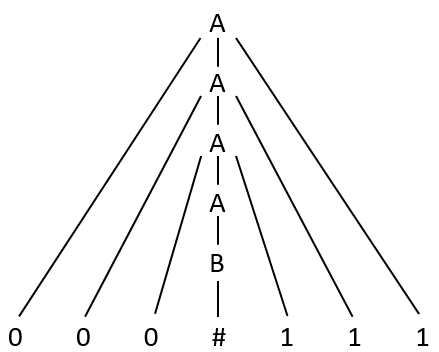
\includegraphics[width=5cm]{figures/derivacni_strom.PNG}
\caption{Derivačný strom gramatiky $\mathcal{G}_1$ pre reťazec \textit{000\#111}}
\label{fig:derivacni_strom}
\end{center}
\end{figure}

Množina všetkých reťazcov, ktoré je možné generovať týmto spôsobom sa nazýva jazyk gramatiky $L$. Jednoduchým pohľadom na gramatiku $G_1$ je možné zapísať jazyk gramatiky ako $L(G_1) \in \{0^n\#1^n | n \geq 0\}$. Všetky jazyky generované bezkontextovou gramatikou sa nazývajú \textbf{bezkontextové jazyky}.

\begin{definice}[\textbf{Jazyk generovaný gramatikou}]
Povedzme, že slovo $\omega \in \Sigma^*$ je \textit{generované} gramatikou $\mathcal{G}$, ak existuje derivácia $S\Rightarrow_\mathcal{G}^*\omega$.

\textit{Jazyk $L(\mathcal{G})$ generovaný} gramatikou $\mathcal{G}$ sa skladá zo všetkých slov generovaných gramatikou $\mathcal{G}$, tj.
\begin{center}
$L(\mathcal{G}) = \{\omega \in \Sigma^* | S \Rightarrow_\mathcal{G}^* \omega\}$.\cite{demlova:gramatiky}
\end{center}
\end{definice}

\subsection{Backus-Naur Form notácia}\label{BNF}
Pri popisovaní jazyka mnohých programovacích jazykov, protokolov alebo formátov sa vo svojej špecifikácii používa zápis pomocou Backus-Naur Form (\nom{BNF}{Backus-Naur Form}) notácie.\cite{might:languages} 

Každé pravidlo v BNF má nasledujúcu štruktúru:
\begin{center}
\textit{<neterminál> ::= výraz}
\end{center}

Všetky netreminály v BNF sa zapisujú do špicatých zátvoriek \textit{< >}, či už sú použité na pravej alebo ľavej strane pravidla. Výraz sa môže obsahovať terminály aj neterminály a je definovaný ich spojením alebo výberom. Symboly vo výraze postavené vedľa seba určujú postupnosť symbolov a použitie znaku vertikálnej lišty určuje výber zo symbolov.

\subsection{Rozšírená Backus-Naur Form notácia}\label{EBNF}
Pre zjednodušenie zápisu gramatiky a aby bolo možné jednoduchšie definovať určité typy pravidiel, vznikla kolekcia rozšírení k Backus-Naur Form notácii (\nom{EBNF}{Extended Backus-Naur Form}), ktorá bola štandardizovaná ako ISO/IEC 14997\cite{ISO14977}. Terminály môžu byť vyjadrené konkrétnym postupom znakov v úvodzovkách alebo pomocou triedy literálov, ktorú je možné zapísať pomocou regulárneho výrazu. Priraďovací znak pravidla je zmenený z ::= na jednoduché = a vynecháva sa zápis špicatých zátvoriek okolo neterminálov. Tieto malé syntaktické zmeny nie sú tak dôležité ako dodatočné operácie EBNF, ktoré sa môžu použiť vo výraze.

\textbf{Nepovinnosť} -- Použitím hranatých zátvoriek okolo výrazu \textit{[výraz]} sa indikuje možnosť použitia tohto výrazu v sekvencii. Jednoduchšie povedané, výraz môže, ale nemusí byť použitý vo výslednej sekvencii. Toto pravidlo je taktiež možné zapísať pomocou znaku ?. Príklad: 
\begin{center}
term = ["\text{-}"] factor\\
term = "\text{-}"? factor
\end{center}

\textbf{Zlučovanie} -- Aby bolo možné identifikovať prioritu sekvencie symbolov, EBNF používa klasické zátvorky, čím jednoznačne definuje poradie výrazov. V príklade je zapísaná gramatika, ktorá prijíma matematické sčítanie a odčítanie:
\begin{center}
expr = term ("\text{+}" \text{|} "\text{-}") expr
\end{center}

\textbf{Opakovanie} -- Použitím zložených zátvoriek okolo výrazu \textit{\{výraz\}} je možné indikovať opakovanie výrazu. To znamená, že výraz sa nemusí v sekvencii vyskytovať, ale zároveň môže byť nekonečne krát za sebou. Toto pravidlo je taktiež možné zapísať pomocou znaku *. Príklad:
\begin{center}
args = arg \{"," \text{ }arg\}\\
args = arg ("," \text{ }arg)$^*$
\end{center}

\textbf{Spájanie} -- Namiesto toho aby sa autor gramatiky spoliehal na postavenie výrazov vedľa seba, má možnosť spájať výrazy aj pomocou znaku čiarky.

Každú gramatiku zapísanú cez EBNF je možné taktiež zapísať pomocou BNF, to ale vedie k omnoho obsiahlejšiemu množstvu definičných pravidiel. V nasledujúcich príkladoch sú znázornené dva rôzne zápisy  gramatiky v EBNF  z kapitoly \ref{CFG}:
\begin{center}
\begin{tabular}{p{0.25\textwidth}}
A = ("0" \text{ A} "1") | B\\
B = "\#"\\\\

A = ("0")$^*$ "\#" \text{ (}"1")$^*$
\end{tabular}
\end{center}

\subsection{Parsing Expression Grammar}
\nomExpl{PEG}{Parsing Expression Grammar} poskytuje alternatívu na popisovanie strojovo orientovanej syntaxi, ktorý rieši problém nejednoznačnosti tým, že ju nepodporuje už od začiatku. Zápis PEG je veľmi podobný zápisu gramatiky pomocou EBNF. Taktiež priamo podporuje veci, ktoré sa bežne používajú, ako sú rozsahy znakov (triedy znakov). Má aj niektoré rozdiely, ktoré v skutočnosti nie sú pragmatické, ako napríklad použitie formálnejšieho symbolu šípky ($\leftarrow$) pre priradenie, namiesto bežnejšieho symbolu rovníc (=). 

Problém nejednoznačnosti spočíva v možnosti zparsovať jeden vstupný reťazec viacerými spôsobmi. Ak by CFG parser spracovával takýto reťazec, mal by v takomto prípade problém. Nakoľko CFG spracováva možnosti pravidiel nedeterministicky, pri parsovaní nejednoznačného vstupu vráti chybu, pretože nevie ktorá zparsovaná možnosť je správna. Na druhú stranu pre PEG riadi výber možností pomocou \textit{prioritnej voľby}, a preto pri parsovaní nejednoznačného vstupu vždy použije prvú možnosť, ktorá je akceptovateľná \cite{ford2004parsing}. Nevýhoda tohto prístupu je v tom, že pri písaní PEG je potreba dbať na správne poradie, inak by mohli vzniknúť pravidlá, ktoré nikdy nebudú vyhovovať. V nasledujúcom príklade slovo \textit{doge} nebude nikdy vyhovovať, nakoľko slovo \textit{dog} je na prvom mieste a bude ihneď vybrané.

\begin{center}
word $\leftarrow$ 'dog' / 'doge'
\end{center}

\section{Parsovanie pomocou regulárnych výrazov}
Regulárne výrazy (\ref{regexp}) poskytujú možnosť zápisu regulárnych jazykov, ktorých fungovanie je postavené na deterministických konečných automatoch (\ref{DFA}).

O regulárnych výrazoch sa často hovorí, že by nemali byť použité na parsovanie. Nie vždy to ale je pravda, pretože je možné použiť regulárne výrazy na parsovanie jednoduchých vstupov. Niektorí programátori nepoznajú iné možnosti a snažia sa všetko parsovať s použitím regulárnych výrazov aj keď by nemali. Výsledkom toho je séria regulárnych výrazov spojených v jeden, čím sa parsovanie môže jednoducho stať vysoko náchylným k chybám.

Parsovanie pomocou regulárnych výrazov je naozaj možné, ale iba pre regulárne jazyky. Pokiaľ sa v jazyku, ktorý sa snažíme parsovať, objavia vnorené alebo rekurzívne elementy, nejedná sa už o regulárny jazyk, ale o jazyk \textit{bezkontextový} (\ref{CFG}). Parsovanie takéhoto jazyka pomocou regulárneho výrazu by spôsobilo degenerovanú slučku \cite{ford2004parsing}. 
% Väčšina programovacích jazykov spadá pod bezkontextové jazyky, a preto nie je možné tieto jazyky parsovať regulárnymi výrazmi.

\section{Štruktúra bezkontextových parserov}
Syntaktickej analýze spravidla predchádza \textit{lexikálna analýza}, pri ktorej sa vstupný reťazec rozdeľuje na postupnosť lexikálnych symbolov (lexémov). V programovacích jazykoch sa taktiež nazývajú \textbf{tokeny} a definujú identifikátory, literály (čísla, reťazce), kľúčové slová, operátory, oddeľovače a pod. Pre parser sú tokeny ďalej nedeliteľné stavebné jednotky, ktoré používa pri interpretácií vstupných dát. Program vykonávajúci túto úlohu sa nazýva štrukturálny analyzátor, no v programovaní sa častejšie narazí na výraz \textbf{lexer} alebo \textbf{tokenizer} bližšie popísaný v kapitole \ref{lexer}. 

V kontexte parsovania sa slovo parser môže odkazovať na program, ktorý vykonáva celý proces, ale aj na správny parser (syntaktický analyzátor), ktorý analyzuje tokeny vytvorené lexerom. Dôvodom toho je, že parser sa stará o najdôležitejšiu a najťažšiu časť celého procesu parsovania. Lexer hrá v procese parsovania iba úlohu pomocníka na uľahčenie práce parseru.

Parsre sú významnou súčasťou kompilátorov alebo interpreterov programovacích jazykov, no samozrejme môžu byť súčasťou aj rôznych typov programov. Čo sa týka parsovania programovacích jazykov, parser dokáže určiť iba syntaktickú korektnosť parsovaného výrazu. Výstup parseru je ale základom pre zistenie sémantickej korektnosti.

\subsection{Lexer}\label{lexer}
Lexery zohrávajú dôležitú  rolu pri parsovaní, pretože transformujú počiatočný vstup na jednoduchšie spracovateľnú formu pre parser. Napísanie gramatiky pre lexer je zvyčajne jednoduchušie, nakoľko nie je nutné riešiť vymoženosti bezkotextového jazyka ako je napríklad opakovanie, rekurzia a podobne.

Jedna z veľmi dôležitých úloh lexera je vysporiadanie sa z medzerami v parsovanom výraze. Vo väčšine prípadov chceme, aby prázdne medzery boli lexerom odstránené. Ak by sa tak nestalo, znamenalo by to, že by sa s nimi musel vysporiadať samotný parser. To by znamenalo ich kontrolu pri každom jednom použitom tokene, čo by sa rýchlo stalo nepríjemným.

Existujú prípady, kedy to nemôžeme urobiť, pretože medzery sú pre daný jazyk relevantné, ako napríklad v prípade Pythonu, kde sa používa identifikácia bloku kódu a je nutné určiť, ktoré medzery sú pre parser dôležité. Aj napriek tomu je zvyčajne lexer zodpovedný za riešenie problému, ktorá medzera je relevantná a ktorá nie. Napríklad pri parsovaní Pythonu chceme, aby lexer overil, či medzery definujú odsadenie (relevantná) alebo medzery medzi slovami (irelevantná). \cite{tomassetti:parsing}

Lexer prečíta vstupný reťazec a rozdelí ho na predom definované typy tokenov. Na definíciu týchto typov sa používajú regulárne výrazy, nakoľko rozdelenie na tokeny spadá pod problém regulárnej gramatiky. Ako už bolo spomenuté na spracovanie regulárnej gramatiky sa používa algoritmus pre DFA(\ref{DFA}).

\begin{figure}[H]
\begin{center}
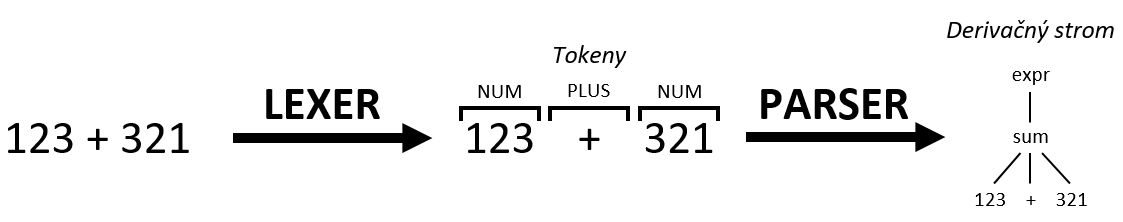
\includegraphics[width=14cm]{figures/lexer_parser.PNG}
\caption{Spracovanie reťazca \textit{123 + 321} lexerom a parserom}
\label{fig:lexer_parser}
\end{center}
\end{figure}

Pre príklad z obrázku \ref{fig:lexer_parser}  máme dva typy tokenov. \textbf{NUM} vyjadrujúci akékoľvek prirodzené číslo a \textbf{PLUS} vyjadrujúci znak súčtu (+). Keď sa lexer bude snažiť analyzovať reťazec \textbf{123 + 321}, bude čítať znaky \textit{1,2,3} a potom znak medzery. V tomto momente lexer rozpozná, že postupnosť znakov \textit{123} súhlasí z definíciou tokenu typu NUM. Následne prečíta znak \textit{+}, ktorý sa zhoduje s druhým typom tokenu PLUS a nakoniec objaví posledný token typu NUM. Takto definované tokeny použije parser na vyhodnotenie výsledného výrazu. Bezkontextová gramatika pre takýto parser by mohla vyzerať nasledovne:

\begin{center}
\begin{tabular}{p{0.35\textwidth}}
\textbf{sum} = NUM \{PLUS NUM\}
\end{tabular}
\end{center}

Vzhľadom na to, že lexery sú takmer výlučne používané v spojení s parsermi, je nutné si určiť hranicu, kde končí práca lexeru a kde začína práca parseru. Táto hranica nemusí byť vždy jasná a všetko to závisí na konkrétnej potrebe programu, pre ktorý je parser vytváraný. Pre príklad si môžeme predstaviť program, ktorý parsuje vstup obsahujúci IP adresu. Pokiaľ programu stačí poznať hodnotu IP adresy, tak je možné vytvoriť token v lexeru, ktorý popisuje celý formát IP adresy a parser pri svojej analýze použije iba tento token. 
\begin{center}
IPv4 = [0-9]+ "."\text{ [}0-9]+ "."\text{ [}0-9]+ "."\text{ [}0-9]+
\end{center}

Ak by bol problém zložitejší a program by chcel analyzovať IP adresu a zistiť z nej informácie, ako napríklad krajinu, bude parser potrebovať jednotlivé hodnoty IP adresy samostatne. V tomto prípade lexer rozdelí IP adresu na dva druhy tokenov (číslo a bodka).

\begin{center}
\begin{tabular}{p{0.65\textwidth}}
\color{editorGray}{/* Lexer */}\\
DOT   = "\text{.}"\\
OCTEC = [0-9]+\\
\color{editorGray}{/* Parser */}\\
ipv4  = OCTET DOT OCTET DOT OCTET DOT OCTET
\end{tabular}
\end{center}

\section{Typické problémy parsovania}
Pri definovaní gramatiky pre parsre existuje niekoľko typických problémov, s ktorými sa jednotlivé parsre musia vysporiadať. 

\subsection{Chýbajúci token}
Častým problémom v gramatikách sú chýbajúce resp. nedefinované tokeny. V niektorých gramatikách sa v rámci lexeru zadefinuje iba časť tokenov ako napríklad

\begin{center}
\begin{tabular}{p{0.3\textwidth}}
\color{editorGray}{/* Lexer */}\\
NAME = [a-zA-Z]+\\
\color{editorGray}{/* Parser */}\\
greeting = "Hello"{ NAME}
\end{tabular}
\end{center}

Token "Hello"{ }nie je pre parser definovaný. Niektoré nástroje na parsovanie sa dokážu s týmto problémom vysporiadať tým, že si sami vygenerujú definíciu pre tieto tokeny, čím zároveň ušetria užívateľovi trochu času \cite{tomassetti:parsing}.

\subsection{Pravidlá s ľavou rekurziou}\label{left-recursion-rule}
V rámci bezkontextových gramatík sa často využíva ľavá rekurzia na definovanie zľava asociatívnych operácií. Tento problém sa najčastejšie rieši v rámci Top Down parserov (viď kapitola \ref{parsing-alg-basics}) s rekurzívnym zostupom (viď kapitola \ref{recursive-descent}). 

Pravidlá s ľavou rekurziou sú také pravidlá, ktoré začínajú s referenciou samy na seba, ako napríklad $A \rightarrow A\alpha$. Do toho problému spadá taktiež nepriama ľavá rekurzia, čo znamená že referencia na samého seba sa objaví v rámci iného pravidla, ako napríklad:

\begin{center}
\begin{tabular}{p{0.15\textwidth}}
$A \rightarrow B\alpha$\\
$B \rightarrow A\beta$\\
\end{tabular}
\end{center}

Predpokladajme, že sa snažím zparsovať pravidlo $A$ na danom mieste vo vstupnom reťazci. Ak by sme na to použili Top Down parser, ktorý pracuje z ľava do prava, našou prvou podúlohou by bolo parsovať pravidlo $A$ na tom istom mieste \cite{moore2000removing}. Takto sa okamžite dostávame do nekonečnej slučky. Rovnaký problém nastane aj s použitím gramatiky, ktorá obsahuje nepriamu ľavú rekurziu, kde sa do nekonečnej slučky dostaneme prechodom cez viac pravidiel.

V teórii, obmedzenie na bezkontextové gramatiky bez ľavej rekurzie nepridáva žiadne obmedzenie na jazyk, ktorý sa snažíme popísať gramatikou. Existujú pravidlá, pomocou ktorých sa dá ľavá rekurzia odstrániť. V zásade každá bezkontextová gramatika obsahujúca ľavú rekurziu môže byť transformovaná na gramatiku bez ľavej rekurzie \cite{moore2000removing}.

% \textbf{Note: moznost pridat priklad odstranovania lavej rekurzie}
% https://tomassetti.me/guide-parsing-algorithms-terminology/#typicalGrammarIssues

    \chapter{Parsovacie algoritmy}
    \chapter{MySQL DDL parser}
Na základe dôvodov popisovaných v poslednej kapitole, som sa na implementáciu DDL parseru pre MySQL rozhodol použiť nástroj ANTLR verzie 4. Tento nástroj je aktuálne vo svete asi najpoužívanejší a prináša veľké množstvo výhod, ktoré uľahčujú implementáciu aj následne ladenie parsovacích programov.

\section{Základy ANTLR v4}

Štvrtá verzia ANTLR má niektoré dôležité nové možnosti, ktoré znižujú učiacu sa krivku a umožnuje vytvárať gramatiky a jazykové aplikáciie oveľa jednoduhšie. Najdôležitejšou výhodou je, že ANTLR v4 akceptuje každú gramatiku, ktorú mu poskytnete (s výnimkou týkajúcou sa nepriamej ľavej rekurzie). ANTLR prekladá vašu gramatiku do spustiteľného, ľudsky čitateľného analytického kódu, do ktorého keď zadáte platný vstupný reťazec, parser vždy rozpozná vstup správne nezávisle na komplikovanosti gramtiky.

V rámci tejto sekcie sú popísané základné informácie potrebné na pochopenie toho, ako s ANTLR pracovať. Na získanie podrobnejších alebo viac detailných informácií doporučujem knihu \textit{The Definitive ANTLR4 reference}\cite{definitiveANTLR} napísanú autorom ANTLR nástroja.

\subsection{Nastavenie ANTLR}
ANTLR sa skladá z dvoch častí: Nástroja na generovanie lexeru a parseru z gramatiky a knižnice potrebnej na beh parseru.

Nástroj na generovanie je rovnaký nezávisle na výstupnom jazyku generovaného lexeru a parseru, a pre samotný beh parseru nie je potrebný. Využijú ho užívatelia, ktorý vytvárajú, alebo upravujú gramatiku. Je to vlastne program napísaný v programovacom jazyku Java, a preto je nutné na prácu s ním mať nainstalovanú aspoň Javu 1.7. Inštalácia ANTLR spočíva v stiahnutí napsledy zverejneného java archívu\footnote{\url{http://www.antlr.org/download.html}}, alebo jeho vybuildením zo zdrojových kódov dostupných v GitHub repositáru\footnote{\url{https://github.com/antlr/antlr4}}. 

Kroky nutné na nainštalovanie ANTLR nástroja:
\begin{enumerate}
\item Nakopírovať stiahnutný nástroj na miesto kde sú uchovávané java knižnice tretích strán.
\item Pridať cestu k nástroju do systemových premenných.
\item Na zjednodušenie používania vytvriť spúštací script a vytvoriť naň alias.
\end{enumerate}
Konkrétne príklady inštalačných krokoj je možné si pozrieť v prílohách \ref{install:windows} pre Windows a \ref{install:linux} pre Linux a Mac OS.

Vstupom pre ANTLR nástroj je súbor s príponou \textit{.g4}, ktorý obsahuje gramatiku jazyka(viď kapitola \ref{antlr_grammar}), pre ktorý bude analyzátor vygenerovaný. príkaz na vygenerovanie lexeru a prseru z definovanej gramatky vyzerá následovne.
\begin{center}
\textit{antlr4 <options> <grammar-file-g4>}
\end{center}

Prvým dôležitým nastavením pri generovaní je možnosť zvoliť si cieľový jazyk vygenerovaného parseru. Prednastavným výstupným jazykom je Java, no ANTLR podpouje aj Python, JavaScript a C\#. Na prechádzanie sparsovaného stromu ANTLR v základe generuje listener objekt, ktorý poslúcha na události vznikajúce pri príchode aj pri odchode z uzlu stromu. Ak užívateľ preferuje použitie visitor paternu pri prechádzaní stromom, je možné ANTLR nástroju nastaviť generovanie visitor objektov.

\subsubsection{Maven}
Pre projekty, ktoré využívajú Maven\footnote{\url{https://maven.apache.org/}} na riadenie a správu buildov aplikácii, je možné túto správu využiť aj pre nastavenie ANTLR.

Prvým krokom je si v \textit{pom.xml} nadefinovať závisosť na \textit{antlr4-runtime}, ktorý je potrebný na beh vygenerovaného parseru.

\begin{lstlisting}[language=XML, frame=none, numbers=none]
<dependency>
    <groupId>org.antlr</groupId>
    <artifactId>antlr4-runtime</artifactId>
    <version>4.7</version>
</dependency>
\end{lstlisting}

Ako druhý krok, je nutné nastaviť maven plugin, pomocou ktorého bude ANTLR generovať parser z poskytnutej gramatiky počas buildu aplikácie. Tento plugin v základe očakáva \textit{.g4} súbory v priečinku \textit{src/main/antlr4}. Túto cestu je možné ručne definovať pomocou configuračného parametru \textit{sourceDirectory}.

\begin{minipage}{\linewidth}
\begin{lstlisting}[language=XML, frame=none, numbers=none]
<plugin>
    <groupId>org.antlr</groupId>
    <artifactId>antlr4-maven-plugin</artifactId>
    <version>4.7</version>
    <configuration>
        <sourceDirectory>${antlr.source.directory}</sourceDirectory>
    </configuration>
    <executions>
        <execution>
            <goals>
                <goal>antlr4</goal>
            </goals>
        </execution>
    </executions>
</plugin>
\end{lstlisting}
\end{minipage}

Na definíciu cieľového balíčka, v ktorom sa budú nachádzať vygenerované súbory, \mbox{ANTLR} použije štruktúru v zdrojovom priečinku. Napríklad ak uvažujeme základný zdrojový priečinok \textit{src/main/antlr4} a cesta k súboru z gramatikou sa bude napríklad:

\begin{center}
\textit{src/main/antlr4/mysql/grammar/MySqlParser.g4}
\end{center}

Vygenerovaný parser sa bude v tomto prípade náchádzať v balíčku \textbf{mysql.grammar}.

\subsection{ANTLR Gramatika}\label{antlr_grammar}
Písanie gramatiky je podobné písaniu softwaru s výnimkou toho, že namiesto funkcií a procedúr sa používajú pravidlá. ANTLR používa zápis gramatiky EBNF notáciu, ktorá je zároveň používana v dokumentáciach programovacích jazykov na popis ich syntaxie. Vďaka nej je možné pri zápise pravidiel používať operácie ako napríklad zlučovanie, opakovanie a nepovinnosť, ktoré sú popísané v kapitole \ref{EBNF}.

Aby bol ANTLR schopný rozpoznať pravidlá pre lexer a parser, je zavedená konvencia na zápis týchto pravidiel. Tá kontroluje, či prvé písmeno pravidla je veľké alebo malé. Síce sa toto pravidlo vzťahuje iba na prvé písmeno, je zvykom definovať názov pravidiel pre lexer iba pomocou veľkých písmen. 

\subsubsection{Pravidlá pre lexer}
Je dôležité mať na pamäti, že lexerove pravidlá sú analyzované v poradí, v akom sa objavujú, a môžu byť nejednoznačné. Typickým príkladom v programovacom jazyku je napríklad to, že názov premennej môže byť akékoľvek slovo s výnimkou na kľúčové slová. Poradie pravidiel rieši nejednoznačnosť tým, že použije prvú zhodu, a preto sú tokeny označujúce kľúčové slová definované ako prvé, zatiaľ čo identifikačné znaky sú uvedené ako posledné. Na lepšie priblíženie tvorby gramatiky pre lexer sa pozrime na príklad:

\begin{lstlisting}[basicstyle=\small, keepspaces=true]
fragment NUMBER           : [0-9]+ ;
DECIMAL_NUMBER       : NUMBER ',' NUMBER ;
WHITESPACE                 : ' ' -> skip ;
\end{lstlisting}

Tento príklad zobrazuje tri typy pravidiel, ktoré sa používajú na vytvorenie gramatiky pre lexer. V prvom pravidle je možné vidieť kľúčové slovo \textbf{fragment}, ktoré definuje prepouživateľné bloky pre pravidlá lexeru. Vďaka definovaniu fragmentu \textit{NUMBER}, je následné možné tento fragment použiť pri definovaní pravidla \textit{DECIMAL\_NUMBER}. Ak by v gramatike existovali definície na fragmenty, ktoré neboli použité na definovanie nejakého pravidla, pre lexer jednoducho nemajú žiadny efekt. Je dôležité si uvedomiť, že fragment sa neberie ako pravidlo lexeru, z čoho vyplýva, že ak by sme pomocou lexeru vytvoreného gramatikou s príkladu chceli analyzovať číslo bez desatinej čiarky, nepodarilo by sa nám to. Aby lexer podporoval aj tento príbad, je nutné upraviť pravidlo na:

\begin{lstlisting}[basicstyle=\small]
DECIMAL_NUMBER : NUMBER (',' NUMBER)? ;
\end{lstlisting}

Najviac zaujímavým pravidlom je pravidlo definujúce medzery (\textit{WHITESPACE}). Zaujímave je z dôvodu, že predstavuje možnosť ako ANTLR-u indikovať, že má niečo ignorovať. Vďaka tomuto pravidlo sa náramne zjednoduší piísanie pravidiel pre parser. Ak by takého pravidlo neexistovalo, musel by to autor gramatiky zahrnúť medzi každú podskupinu pravidiel parseru. ako napríklad:
\begin{lstlisting}[basicstyle=\small]
sum  : WHITESPACE* NUMBER WHITESPACE* '+' WHITESPACE* NUMBER;
\end{lstlisting}

Tento princíp sa typicky aplikuje aj na komentáre. Tie sa taktiež môžu objaviť kdekoľvek a väčšinou autora pri parsovaní nezujímajú, takže sa jednoducho ignorujú.

\subsubsection{Dostupné gramatiky}
Kľučovou výhodou ANTLR v4 je dostupnosť obrovského množstva vytvorených gramatík od autorov z celého sveta, ktoré sú združené v rámci ANTLR GitHub repozitáru\footnote{\url{https://github.com/antlr/grammars-v4}}. Pre tieto gramatiky neexistuje žiadna globálna licencia. Každá z gramaík má svoju vlastnú licenciu. Súčasťou tejto kolekcie je aj gramatika pre MySQL, ktorá je vytvorená na základe dokumentácie pre MySQL verzie 5.6 a 5.7, čo presne vyhovuje potrebám projektu Debezium. MySQL gramatika je vydaná pod licenciou MIT\footnote{MIT licencia je jedna z najmenej reštriktívnych open source licencií. Ktokoľvek môže takto licencovaný program bez obmedzenie používať a šíriť, pokiaľ z programu neodstráni kopiu licencie a meno autora.}.

\subsection{Ukážková implementácia}
% https://gist.github.com/mattmcd/5425206
Ako ukážkovú implementáciu použijeme príklad na parsovanie pozdravu. Prvým krokom implementácie je definícia gramatiky (viď ukážka \ref{code:hello_grammar}). V tomto prípade o je veľmi jednoduchá gramatika o jednom pravidle \textit{greeting}, ktoré na prvom mieste očakáva slovo \textit{hello} následované akýmkoľvek reťazcom skladajúcim sa z malých písmen abecedy.

\lstinputlisting[caption=Ukážková gramatika Hello, 
            label=code:hello_grammar,
            keepspaces=true]
            {code/6/hello_grammar.tex}

Z tejto gramatiky ANTLR vygeneruje \inlinecode{HelloParser}, \inlinecode{HelloLexer}, rozhranie \inlinecode{HelloListener} a jeho základnú (prázdnu) implementáciu \inlinecode{HelloBaseListener}. Použitím je možné počúvať príchod a odchod na pravidlá gramatiky. Implementujeme si vlastný \inlinecode{HelloListenerCustom} pomocou ktorého budeme reagovať na nami zvolené události. V tomto prípade to je výpis na systemový výstup pri príchode aj odchode na pravidlo \textit{greeting} (viď ukážka \ref{code:hello_listener}).

\lstinputlisting[language=Java2,
			caption=Ukážková implementácia HelloListener.java, 
            label=code:hello_listener]
            {code/6/HelloListener.java}

Posledným krokom je implementovať Main aplikáciu, ktorá inicializuje \inlinecode{HelloLexer}, \inlinecode{HelloParser} a spustí samotné parsovanie (viď ukážka \ref{code:hello_main}). \inlinecode{HelloLexer} as incializuje pomocou prúdu znakov reprezentovaných \inlinecode{CharStream} objektom. Použitím lexeru si vytvoríme prúd tokenov \inlinecode{CommonTokenStream}, ktorým inicializujeme \inlinecode{HelloParser}. Zavolaním príkazu na riadku 10 ukážky \ref{code:hello_main} spustíme proces parsovania, ktorého vstupom je sparsovaný strom. osledným krokom je prechod stromu pomocou \inlinecode{ParseTreeWalker} triedy, ktorej prradíme nami vytvorený \inlinecode{HelloListenerCustom}. Náš \inlinecode{HelloListenerCustom} je možné priradiť aj parseru, vďaka čomu by sme mohli odchytávat události už počas toho, ako sa vygenerovaný parser snaží vytvoriť sparsovaný strom. V takomto prípade je ale nutné počítat zo situáciami, že aktuálne sparovaný kontext nie je úplny a taktiež nie je zaručené, že pravidlo bude obsiahnuté vo výslednom sparsovanom strome. 

\begin{minipage}{\linewidth}
\lstinputlisting[language=Java2,
			caption=Ukážková implementácia Main.java, 
            label=code:hello_main]
            {code/6/Hello.java}
\end{minipage}

\section{Návrh DDL parseru}
Pri návrhu nového generovaného DDL parseru pomocou ANTLR, je dôležité brať v úvahu aktuálny design projektu Debezium a implementáciu stávajúceho parseru. Primárnou snahou je prepoužiť čo možno najväčšiu časť aktuálnej implementácie, ktorú už niekoľko projektov využíva. Počas návrhu taktiež prihliadam na budúcnosť, ktorá nasvedčuje tomu, že projekt Debezium má v pláne podporovať väčšie množstvo DBMS, ktorých prípadne DDL parsery budú taktiež využívať ANTLR nástroj. Práve na základe tejto skutočnosti je snaha zgeneralizovať čo najväčšiu časť novej implementácie.

\subsection{Aktuálny design}\label{old_design}
Štruktúra projektu Debezium je členená do viacerých modulov. Každý konektor pre jednotlivé DBMS je implementovaný v samostatnom module. V kontexte DDL parsovania MySQL sú významné dva moduly:
\begin{itemize}
\item \textbf{debezium-core} modul, v ktorom sa nachádza implementácia spoločná pre všetky databázové systémy.
\item \textbf{debezium-connector-mysql} modul, ktorý je závislý na \textit{debezium-core} module. Súčasťou modulu je celá implementácia špecifická pre MySQL databázový systém, ktorej súčasťou je aj aktuálny DDL parser, ktorý má byť nahradený.
\end{itemize}

MySQL je akuálne jediným Debziom podporovaným databázovým systémom, v rámci ktorého sa parsuju DDL. Pravdepodobne z tohto dôvodu nebola implementácia dostatočne generalizovaná a mnohé funckionality, ktoré do budúcna budú využívať aj iné typy DDL parserov neboli implemenované v rámci \textit{debezium-core} modulu.

Vstupným bodom pre DDL parser je komponenta \inlinecode{MySqlSchema}, ktorá zaznamenáva históriu schémat pre databáze hostované na MySQL. V rámci tejto komponenty sa inicializuje \inlinecode{MySqlDdlParser}, ktorý dedí od \inlinecode{DdlParser}. Diagram na obrázku \ref{fig:class_diagram_old} znázornuje aktuálnu závislosť tried a verejných metód, ktoré sú podstatné pre MySQL DDL parser.

\begin{figure}[H]
\begin{center}
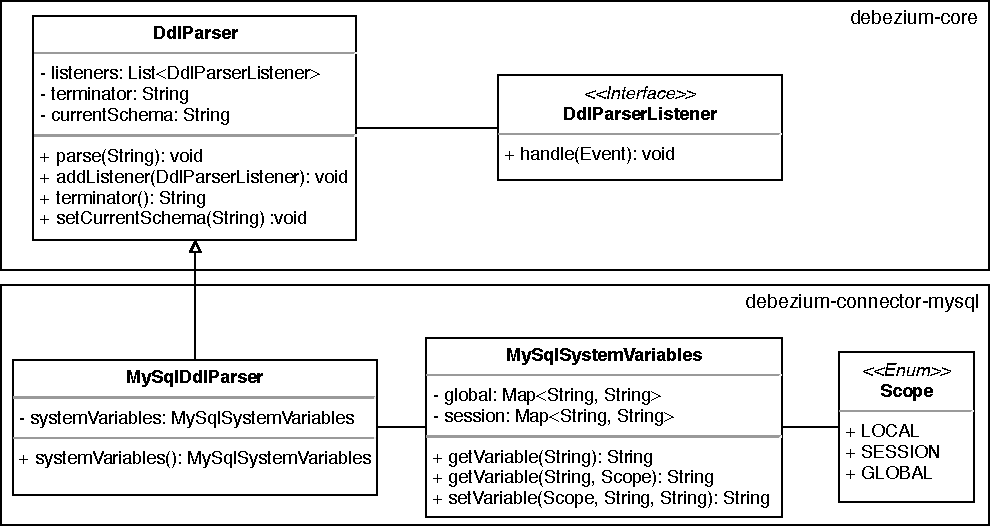
\includegraphics[width=10cm]{figures/Old_modules.pdf}
\caption{Diagram tried aktuálneho návrhu MySQL DDL parseru}
\label{fig:class_diagram_old}
\end{center}
\end{figure}

Všetky verejné metódy, ktoré obsahuje \inlinecode{DdlParser} a \inlinecode{MySqlDdlParser} predstavujú API parseru, ktoré je volané komponentou \inlinecode{MySqSchema}. 

Stávajúci návrh je viac než nedostačujúci pre možnosť rozšírenia, či už novým parserom pre MySQL databázový systém, alebo parserom pre ktorý koľvek iný DBMS. Na prvý pohľad je napríklad možné vidieť absenciu rozhrania pre \inlinecode{DdlParser}. Bližší pohľad na jedotlivé triedy z obrázku \ref{fig:class_diagram_old} nám načrtne obraz na vylepšenie tohto návrhu.

\inlinecode{DdlParser} trieda má aktuálne predstavovať základ pre všetky DDL parsre. Obsahuje implementáciu kľúčových metód, ktoré riešia: 
\begin{itemize}
\item Nastavenie DDL parseru ako napríklad, či sa majú parsovať dotazy pre náhľady tabuliek, ktoré scháma resp. databáza je aktuálne sledovaná a podobne.
\item Signalizáciu zmien nad databázou, ktoré boli počas parsovania detekované.
\item Spoločné pomocné metódy, ako napríkad metóda na vyseparovanie reťazca, ktorý je obklopený úvodzovkami a mnohé ďalšie.
\end{itemize}

Súčasťou \inlinecode{DdlParser} triedy je ale aj implementácia základnej parsovacej logiky a parsovanie konkrétnych typov reťazcov, u ktorých sa predpokladalo, že ich bude možné prepoužiť aj v rámci ďalších implementácií ddl parserov.

Trieda \inlinecode{MySqlDdlParser} predstavuje implementáciu DDL parseru. Táto trieda je už špecifická pre MySQL databázový systém, a preto nie je možné jú ďalej generalizovať. Jediným problém, ktorý u tejto implementácie nastal, je trieda \inlinecode{MySqlSystemVariables}, ktorá udržuje systémove premenné na úrovni priestoru definovaného pomocou enumu \inlinecode{Scope}. Autor túto funckionalitu implementoval ako súčasť MySQL, no správne by mala byť taktiež generalizovaná, nakoľko každý DBMS má svoje vlastné systémové premenné.

\subsection{Úprava aktuálneho designu}
Na základe nedokonalostí zistených v aktuálnom návrhu DDL parsrov, je potrebné vykonať zmeny v tomto návrhu tak, aby vyhovovali implementácii nového parseru generovaného pomocou ANTLR, ale zároveň zachvovali aktuálne riešenie a prípadnú implementáciu nových DDL parserov týmto "starým"{ }spôsobom.

Prvou zmenou v návrhu je vytvorenie rozhrania pre DDL parsre, ktoré bude definovať možnosť komunikácie pre komponenty, ktoré potrebujú parsovať DDL dotazy. Toto rozhranie bude definovať všetky verejné metódy z tried \inlinecode{DdlParser} a \inlinecode{MySqlDdlParser}. Tým sa dostávame k prvému problému, ktorým sú systemové premenné. Nakoľko nové rozhranie bude súčaťou \textit{debezium-core} modulu, je nutné generalizovať triedu \inlinecode{MySqlSystemVariables}. 

Aktuálna implemenácia triedy \inlinecode{MySqlSystemVariables} obsahuje dve \inlinecode{Map} objekty, ktoré udržiavali hodnoty systémových premenných tak, že na základe hodnoty enumu \inlinecode{Scope} bola zvolená správna mapa z ktorej sa hodnota premennej čítala. Takýto prístup v generovalizovanej verzii nie je možné použiť, nakoľko hodnoty priestoru definovaného enumom \inlinecode{Scope} sú odlišné v závislosti na DBMS. Ukladanie systémových premenných volá po riešní pomocou mapy priradenej k hodnote \inlinecode{Scope} enumu. Enum je ale špeciálny typ objektu v Jave, ktorý nedokáže dediť od iného enumu, čo prináša dilemu spojenú s tým, ako vyriešiť vlastné hodnoty \inlinecode{Scope} pre jednotlivé DBMS? 

Extendovanie enumov je väčšinou zlý nápad, no toto je jeden z prípadov kde to dáva zmysel. Možnosť ako túto situáciu vyriešiť je namiesto enumu \inlinecode{Scope} použiť rozhranie \inlinecode{Scope}. V takomto prípade majú jednotlivé implementácie možnosť vytovrenia vlastného enumu s vlastnými hodnotami kde stačí, aby tento enum implementoval rozhranie \inlinecode{Scope}. \cite{effective_java}

Nakoľko chceme prepoužiť resp. zanechať čo možno najväčiu čast stávajúcej aplikácie, bolo by vhodné vyseparovať z triedy \inlinecode{DdlParser} všetko, čo by mohola používať aj nová implmentácia parseru. Ako bolo popísané v kapitole \ref{old_design}, súčasťou implementácie \inlinecode{DdlParser} sú kľúčové metódy, ktoré nie sú závislé na štýle parsovania, a preto je vhodné ich prepoužiť aj v rámci ANTLR parseru. Vyseparujeme preto túto časť implementáciie do abstraktnej triedy, ktorá bude predstavovať najnutnejší základ pre všetky typy DDL parserov. Všetky ostatné metódy, ponecháme v \inlinecode{DdlParser}. Aby názvoslovie nebolo príliš zmätočné pozostatok triedy \inlinecode{DdlParser} predstavujúci implementáciu základnej parsovacej logiky pre ručné parsovanie nazveme \inlinecode{LegacyDdlParser} a názov \inlinecode{DdlParser} rezervujeme pre novo vytvorené rozhranie DDL parserov.

Pri každej zmene, ktorá nastane nad databázovým modelom uloženým v pamäti sa pomocou události táto zmena signalizuje poslucháčom, ktorý boli priradený DDL parseru. Myšlienka tejto funkcionality ale v stávajúcej implementácii nie je využitá. Jediným poslucháčom je \inlinecode{DdlChanges} trieda, ktorá sa tvári ako poslucháč, ale reálne tak nepracuje. Jeho reakcia na prijatú udalosť spočíva v iba v tom, že si túto událosť pridá do listu událostí, s ktorým sa následne pracuje až po ukončení práce parseru. Nakoľko neexistujú žiadny iný poslucháči, vedenie projektu sa rozhodlo túto funkcionalitu zanechat v rámci \inlinecode{LegcyDdlParser} implementácie, ale nechcelo ju mať v novej implementácii. \inlinecode{DdlChanges} trieda sa teda stane súčasťou abstraktnej implementácie parseeru a prístup k nej bude možný pomocou vystavenej metódy v rámci \inlinecode{DdlParser} rozhrania.

\begin{figure}[H]
\begin{center}
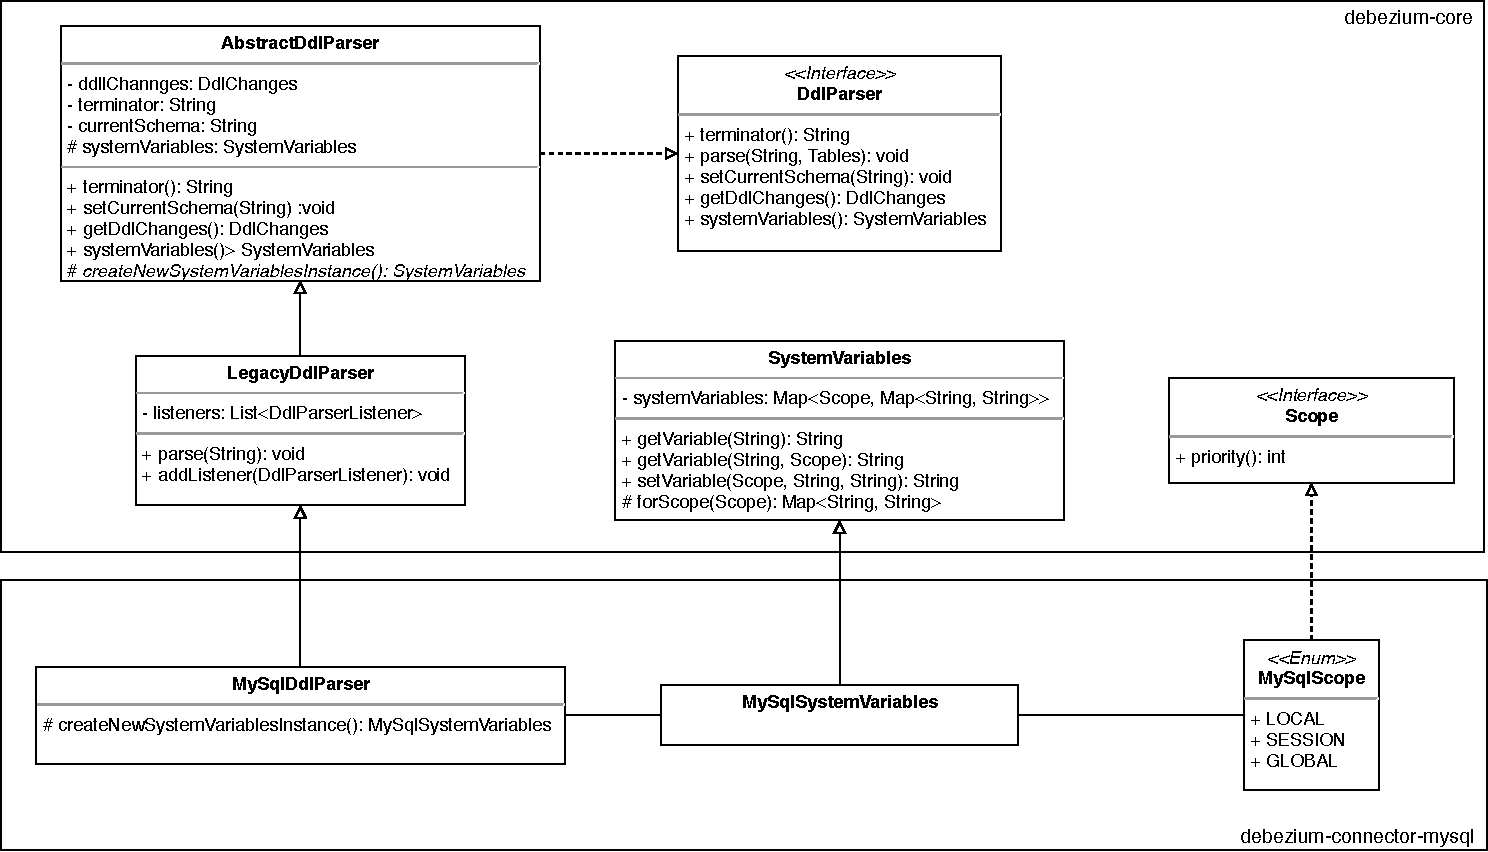
\includegraphics[width=15cm]{figures/New_design.pdf}
\caption{Upravený diagram tried MySQL DDL parseru}
\label{fig:class_diagram_new}
\end{center}
\end{figure}

\subsection{ANTLR DDL parser design}
Úpravou designu aktuálnej implementácie, ktorej výsledok je možné vidieť na obrázku \ref{fig:class_diagram_new} nám zabezpečí možnosť jedoduhšieho návrhu pre DDL parsre generované pomocou \mbox{ANTLR}. Z celého návrhu je nutné nahradiť triedy \inlinecode{LegacyDdlParser} a \inlinecode{MySqlDdlParser} za novú implementáciu. Zachovaním myšlienky na prepoužitie bude opäť návrh obsahovať triedu zo základnou implementáciou ANTLR parserov a konkrétnu implementáciu pre MySQL DBMS.


    \chapter{Záver}
Cieľom tejto práce bolo zanalyzovať možnosti nahradenia existujúceho DDL parseru pre MySQL, ktorý v projekte Debezium odchytáva zmeny v databázoých štruktúrach. Aktuálne riešenie nebolo dostačujúce na spracovanie všetkých možných nuancí jazyka MySQL a náročnosť prípadných úprav rástla z veľkosťou jeho implementácie. V rámci analýzy existujúceho parsru boli objavené nekonzistencie voči MySQL syntaxi, čo znamená, že parser príjmal aj nevalidné SQL dotazy.

Analýzou možností, ako by stávajúci parser mohol byť nahradený sa ukázalo, že parsovanie je teoreticky vyriešený problém, no v praxi sa tento problém stále znovu rieši. To znamená, že existuje vela rôznych algoritmov, každý so silnými a slabými stránkami a stále sa vylepšujú. Pre správnu voľbu parsovacieho algoritmu existuje niekoľko faktorov, ktoré je potrebné brať do úvahy. Najdôležitejším z nich je uvedomiť si, do akého jazyka spadá gramatika, ktorú sa snažíme parsovať. Jazyk MySQL spadá pod bezkontextové jazyky, nakoľko obsahuje možnosti rekurzívnych pravidiel. Vačšina algoritmov, ktorá dokáže parsovať bezkontextové jazyky vyžaduje úpravu gramatiky, ako napríklad odstránenie ľavých rekurzií u LL algoritmov. 

Vďaka neustálemu rozširovaniu možnosí parsovania už existujú nástroje, ktoré dokážu niektoré z týchto úprav vykonať, takže autor gramatiky ich môže ignorovať. Nástroj ANTLR verzie 4, ktorý som si zvolil pre riešenie nového parseru, používa aktuálne najnovší parsovací algoritmus ALL(*), ktorý je postavený na LL algoritmoch a bol vyvinutý v roku 2014 práve autorom nástroja ANTLR. Pri generovaní parseru z gramatiky sa ANTLR dokáže vysporiadať s pravidlami obsahujúcimi priamu ľavú rekurziu, no autor si stále musí dávať pozor na nepriamu ľavú rekurziu.

Pri návrhu implementácie nového parseru, generovaného nástrojom ANTLR sa taktiež ukázali nedostatky v existujúcom návrhu, ktorý nebol dostatočne pripravený na možnosti rozšírenia parsovania iným spôsobom. Z toho dôvodu bolo nutné upraviť aktuálny návrh tak, aby bolo možné využiť čo najväčšiu časť existujúcej implementácie. Projekt Debezium bude v budúcnosti rozširovať podporu databázových systémov, ktoré bude možné sledovať, a preto sa pri návrhu počítalo z použitím ANTLR nástroja pri parsovaní iných DBMS. Základná implementácia, ktorá by mala byť spoločná pre všetky ANTLR parsre je implementovaná v samostatnom module, ktorý sa taktiež stará o generovanie parserov z daných gramatík.

Funkcionalita implementácie nového parseru bola úspešne overená testvacou sadou Debezia. V niektorých prípadoch bolo potrebné túto sadu upraviť a to najmä zo spomínaného dôvodu, že predchádzajúca implementácia povoľovala parsovanie syntakticky nevalidných SQL dotazov. V rámci nového ANTLR parseru boli taktiež implementované opravy nájdených chýb a parsovanie SQL dotazov, ktoré v bývalej implementácii neboli parsované. Na základe týchto novoparsovaných dotazov bola existujúca sada rozšírená. Súčasťou novej sady je taktiež kontrola správnosti gramatiky, ktorá môže byť v budúcnosti upravovaná.

V tejto práci sa mi podarilo zanalyzovať možnosti implementácie generovaného parseru a taktiež takýto parser implementovať pre budúce potreby projektu Debezium. Táto implementácia prináša veľa výhod pre projekt Debezium a to najmä v zmysle údržby parseru a prípadnej implementácie parseru pre iný databázový systém. Analýza jednotlivých sparsovaných dotazov je rozdelená do viacerých tried, čo prináša väčšiu prehľadnosť a jednoduchšiu orientáciu pre vývojarov, ktorí s DDL parserom prídu do styku.
    % \chapter{Pomoc}
\section{Obrázky}
Obrázky jsou vhodným nástrojem pro ilustraci a doplnění textu, používejte je v rozumné míře ať vaše práce nepřipomíná komix. Při hledání/tvorbě obrázků nezapomeňte na to, že u přejatých obrázků musíte odkazovat jejich zdroj a že obrázky by měly být čitelné (typicky .jpg soubory se často rozostří). Dalším častým neduhem jsou obrázky s anglickými popisky v česky psaném textu, pokud to je možné udržte jazyk práce jednotný.

\subsection{Vkládání obrázků}
Obrázky se umísťují do plovoucího prostředí \verb|figure|. Každý obrázek by měl obsahovat \textbf{název} (\verb|\caption|) a \textbf{návěští} (\verb|\label|). Použití příkazu pro vložení obrázku \\\verb|\includegraphics| je podmíněno aktivací (načtením) balíku graphicx příkazem\\ \verb|\usepackage{graphicx}|.

Budete-li zdrojový text zpracovávat pomocí programu \verb|pdflatex|, očekávají se obrázky s příponou \verb|*.pdf|\footnote{pdflatex umí také formáty PNG a JPG.}, použijete-li k formátování \verb|latex|, očekávají se obrázky s příponou \verb|*.eps|.\footnote{Vzájemnou konverzi mezi snad všemi typy obrazku včetně změn vekostí a dalších vymožeností vám může zajistit balík ImageMagic  (http://www.imagemagick.org/script/index.php). Je dostupný pod Linuxem, Mac OS i MS Windows. Důležité jsou zejména příkazy convert a identify.}

\begin{figure}[ht]
\begin{center}

\includegraphics[width=5cm]{figures/LogoCVUT}
\caption{Popiska obrázku}
\label{fig:logo}
\end{center}
\end{figure}

Příklad vložení obrázku:
\begin{verbatim}
\begin{figure}[h]
\begin{center}

\includegraphics[width=5cm]{figures/LogoCVUT}
\caption{Popiska obrazku}
\label{fig:logo}
\end{center}
\end{figure}
\end{verbatim}

\subsection{Kreslení obrázků}
Zřejmě každý z vás má nějaký oblíbený nástroj pro tvorbu obrázků. Jde jen o to, abyste dokázali obrázek uložit v požadovaném formátu nebo jej do něj konvertovat (viz předchozí kapitola). Je zřejmě vhodné kreslit obrázky vektorově. Celkem oblíbený, na ovládání celkem jednoduchý a přitom dostatečně mocný je například program Inkscape.

Zde stojí za to upozornit na kreslící programe Ipe \cite{ipe}, který dokáže do obrázku vkládat komentáře přímo v latexovském formátu (vzroce, stejné fonty atd.). Podobné věci umí na Linuxové platformě nástroj Xfig. 

Za pozornost ještě stojí schopnost editoru Ipe importovat obrázek (jpg nebo bitmap) a krelit do něj latexovské popisky a komentáře. Výsledek pak umí exportovat přímo do pdf.

Další možností je knihovna graphviz, které vykreslí obrázek podle vašeho popisu (kódu), výstup je možný do mnoha formátů (.eps, .jpg, ...).


\section{Tabulky}
Existuje více způsobů, jak sázet tabulky. Například je možno použít prostředí \verb|table|, které je velmi podobné prostředí \verb|figure|. 

\begin{table}
\begin{center}
\begin{tabular}{|c|l|l|}
\hline
\textbf{DTD} & \textbf{construction} & \textbf{elimination} \\
\hline
$\mid$ & \verb+in1|A|B a:sum A B+ & \verb+case([_:A]a)([_:B]a)ab:A+\\
&\verb+in1|A|B b:sum A B+ & \verb+case([_:A]b)([_:B]b)ba:B+\\
\hline
$+$&\verb+do_reg:A -> reg A+&\verb+undo_reg:reg A -> A+\\
\hline
$*,?$& the same like $\mid$ and $+$ & the same like $\mid$ and $+$\\
& with \verb+emtpy_el:empty+ & with \verb+emtpy_el:empty+\\
\hline
R(a,b) & \verb+make_R:A->B->R+ & \verb+a: R -> A+\\
 & & \verb+b: R -> B+\\
\hline
\end{tabular}
\end{center}
\caption{Ukázka tabulky}
\label{tab:tab1}
\end{table}

Zdrojový text tabulky \ref{tab:tab1} vypadá takto:
\begin{verbatim}
\begin{table}
\begin{center}
\begin{tabular}{|c|l|l|}
\hline
\textbf{DTD} & \textbf{construction} & \textbf{elimination} \\
\hline
$\mid$ & \verb+in1|A|B a:sum A B+ & \verb+case([_:A]a)([_:B]a)ab:A+\\
&\verb+in1|A|B b:sum A B+ & \verb+case([_:A]b)([_:B]b)ba:B+\\
\hline
$+$&\verb+do_reg:A -> reg A+&\verb+undo_reg:reg A -> A+\\
\hline
$*,?$& the same like $\mid$ and $+$ & the same like $\mid$ and $+$\\
& with \verb+emtpy_el:empty+ & with \verb+emtpy_el:empty+\\
\hline
R(a,b) & \verb+make_R:A->B->R+ & \verb+a: R -> A+\\
 & & \verb+b: R -> B+\\
\hline
\end{tabular}
\end{center}
\caption{Ukázka tabulky}
\label{tab:tab1}
\end{table}
\begin{table}
\end{verbatim}

A pokud máte svá data v CSV můžete použít některou z knihoven nabízených v   http://texblog.org/2012/05/30/generate-latex-tables-from-csv-files-excel/ 

\section{Odkazy v textu}
\subsection{Odkazy na literaturu}
Jsou realizovány příkazem \verb|\cite{odkaz}|. 

Seznam literatury je dobré zapsat do samostatného souboru a ten pak zpracovat programem bibtex (viz soubor \verb|reference.bib|). Zdrojový soubor pro \verb|bibtex| vypadá například takto:
\begin{verbatim}
@Article{Chen01,
  author  = "Yong-Sheng Chen and Yi-Ping Hung and Chiou-Shann Fuh",
  title   = "Fast Block Matching Algorithm Based on 
             the Winner-Update Strategy",
  journal = "IEEE Transactions On Image Processing",
  pages   = "1212--1222",
  volume  =  10,
  number  =   8,
  year    = 2001,
}

@Misc{latexdocweb,
  author  = "",
  title   = "{\LaTeX} --- online manuál",
  note    = "\verb|http://www.cstug.cz/latex/lm/frames.html|",
  year    = "",
}
...
\end{verbatim}

%11.12.2008, 3.5.2009
\textbf{Pozor:} Sazba názvů odkazů je dána Bib\TeX{} stylem\\ (\verb|\bibliographystyle{abbrv}|). 
%Budete-li používat české prostředí (\verb|\usepackage[czech]{babel}|), 
Bib\TeX{} tedy obvykle vysází velké pouze počáteční písmeno z názvu zdroje, 
ostatní písmena zůstanou malá bez ohledu na to, jak je napíšete. 
Přesněji řečeno, styl může zvolit pro každý typ publikace jiné konverze. 
Pro časopisecké články třeba výše uvedené, jiné pro monografie (u nich často bývá 
naopak velikost písmen zachována).

Pokud chcete Bib\TeX u napovědět, která písmena nechat bez konverzí 
(viz \texttt{title = "\{$\backslash$LaTeX\} -{}-{}- online manuál"} 
v~předchozím příkladu), je nutné příslušné písmeno (zde celé makro) uzavřít 
do složených závorek. Pro přehlednost je proto vhodné celé parametry 
uzavírat do uvozovek (\texttt{author = "\dots"}), nikoliv do složených závorek.

Odkazy na literaturu ve zdrojovém textu se pak zapisují:
\begin{verbatim}
Podívejte se na \cite{Chen01}, 
další detaily najdete na \cite{latexdocweb}
\end{verbatim}

Vazbu mezi soubory \verb|*.tex| a \verb|*.bib| zajistíte příkazem 
\verb|\bibliography{}| v souboru \verb|*.tex|.  V našem případě tedy zdrojový 
dokument \verb|thesis.tex| obsahuje příkaz\\
\verb|\bibliography{reference}|.

Zpracování zdrojového textu s odkazy se provede postupným voláním programů\\
\verb|pdflatex <soubor>| (případně \verb|latex <soubor>|), \verb|bibtex <soubor>| 
a opět\\ \verb|pdflatex <soubor>|.\footnote{První volání \texttt{pdflatex} 
vytvoří soubor s~koncovkou \texttt{*.aux}, který je vstupem pro program 
\texttt{bibtex}, pak je potřeba znovu zavolat program \texttt{pdflatex} 
(\texttt{latex}), který tentokrát zpracuje soubory s příponami \texttt{.aux} a 
\texttt{.tex}. 
Informaci o případných nevyřešených odkazech (cross-reference) vidíte přímo při 
zpracovávání zdrojového souboru příkazem \texttt{pdflatex}. Program \texttt{pdflatex} 
(\texttt{latex}) lze volat vícekrát, pokud stále vidíte nevyřešené závislosti.}


Níže uvedený příklad je převzat z dříve existujících pokynů studentům, kteří 
dělají svou diplomovou nebo bakalářskou práci v~Grafické skupině.\footnote{Několikrát 
jsem byl upozorněn, že web s těmito pokyny byl zrušen, proto jej zde přímo necituji. 
Nicméně příklad sám o sobě dokumentuje obecně přijímaný konsensus ohledně citací 
v~bakalářských a diplomových pracích na KP.} Zde se praví:
\begin{small}
\begin{verbatim}
...
j) Seznam literatury a dalších použitých pramenů, odkazy na WWW stránky, ...
 Pozor na to, že na veškeré uvedené prameny se musíte v textu práce 
 odkazovat -- [1]. 
Pramen, na který neodkazujete, vypadá, že jste ho vlastně nepotřebovali 
a je uveden jen do počtu. Příklad citace knihy [1], článku v časopise [2], 
stati ve sborníku [3] a html odkazu [4]: 
[1] J. Žára, B. Beneš;, and P. Felkel. 
     Moderní počítačová grafika. Computer Press s.r.o, Brno, 1 edition, 1998. 
     (in Czech). 
[2] P. Slavík. Grammars and Rewriting Systems as Models for Graphical User 
     Interfaces. Cognitive Systems, 4(4--3):381--399, 1997. 
[3] M. Haindl, Š. Kment, and P. Slavík. Virtual Information Systems. 
     In WSCG'2000 -- Short communication papers, pages 22--27, Pilsen, 2000. 
     University of West Bohemia. 
[4] Knihovna grafické skupiny katedry počítačů: 
     http://www.cgg.cvut.cz/Bib/library/ 
\end{verbatim}
\end{small}
\ldots{} abychom výše citované odkazy skutečně našli v (automaticky generovaném) seznamu literatury tohoto textu, musíme je nyní alespoň jednou citovat: Kniha \cite{kniha}, článek v~časopisu \cite{clanek}, příspěvek na konferenci \cite{sbornik}, www odkaz \cite{www}.

Ještě přidáme další ukázku citací online zdrojů podle české normy. Odkaz na wiki o frameworcich \cite{wiki:framework} a ORM \cite{wiki:orm}. Použití viz soubor \verb|reference.bib|. V seznamu literatury by nyní měly být živé odkazy na zdroje. V \verb|reference.bib| je zcela nový typ publikace. Detaily dohledal a dodal Petr Dlouhý v dubnu 2010. Podrobnosti najdete ve zdrojovém souboru tohoto textu v komentáři u příkazu \verb|\thebibliography|.

\subsection{Odkazy na obrázky, tabulky a kapitoly}
\begin{itemize}
\item Označení místa v textu, na které chcete později čtenáře práce odkázat, se provede příkazem \verb|\label{navesti}|. Lze použít v prostředích \verb|figure| a  \verb|table|, ale též za názvem kapitoly nebo podkapitoly.
\item Na návěští se odkážeme příkazem \verb|\ref{navesti}| nebo \verb|\pageref{navesti}|.
\end{itemize}

\section{Rovnice, centrovaná, číslovaná matematika}
Jednoduchý matematický výraz zapsaný přímo do textu se vysází pomocí prostředí \verb|math|, resp. zkrácený zápis pomocí uzavření textu rovnice mezi znaky \verb|$|.
Kód \verb|$ S = \pi * r^2 $| bude vysázen takto: $ S = \pi * r^2 $.
Pokud chcete nečíslované rovnice, ale umístěné centrovaně na samostatné řádky, pak lze použít prostředí \verb|displaymath|, resp. zkrácený zápis pomocí uzavření textu rovnice mezi znaky \verb|$$|. Zdrojový kód: 
\begin{verb}
|$$ S = \pi * r^2 $$|
\end{verb}
bude pak vysázen takto:
$$ S = \pi * r^2 $$
Chcete-li mít rovnice číslované, je třeba použít prostředí \verb|eqation|. Kód:
\begin{verbatim}
\begin{equation}
  S = \pi * r^2
\end{equation}
\begin{equation}
  V = \pi * r^3
\end{equation}
\end{verbatim}
je potom vysázen takto:
\begin{equation}
  S = \pi * r^2
\end{equation}
\begin{equation}
  V = \pi * r^3
\end{equation}
\section{Kódy a algoritmy}
\subsection{Zdrojové kódy}
Chceme-li vysázet například část zdrojového kódu programu, hodí se prostředí \verb|verbatim|, které je bez formátování: 
\begin{verbatim}
         (* nickname2 *)
Lego> Refine in1
             (do_reg (nickname1 h));
Refine by  in1 (do_reg (nickname1 h))
   ?4 : pcdata
   ?5 : pcdata
          (* surname2 *)
Lego> Refine surname1 h;
Refine by  surname1 h
   ?5 : pcdata
          (* email2 *)
Lego> Refine undo_reg (email1 h);
Refine by  undo_reg (email1 h)
*** QED ***
\end{verbatim}
nebo se dá použít \verb|listings|, což je package, který umožňuje i syntax higlighting podle jazyka:
\lstset{language=Python} %následuje python kód a použije se python syntax
\begin{lstlisting}
	print 'Hello, world!'
\end{lstlisting}
a umožňuje načíst i přiložené zdrojové soubory:
\lstinputlisting[language=C]{code/hello.c}
\subsection{Algoritmy}
Pokud chcete v práci popsat obecné algoritmy s využitím pseudokódu, můžete použít knihovny \verb|algorithmicx| a \verb|algpseudocode|:
\begin{algorithmic}
\If {$i\geq maxval$}
    \State $i\gets 0$
\Else
    \If {$i+k\leq maxval$}
        \State $i\gets i+k$
    \EndIf
\EndIf
\end{algorithmic}
\section{Zkratky}

V tomto textu používám několik zkratek, třeba 2D\nomenclature{2D}{Two-Dimensional} nebo \nomExpl{KNB}{Killing nanobots}. V úvodní části dokumentu můžete nastavit/upravit příkaz pro zadání zkratky, pokud např. chcete mít význam zkratky pod čarou. Všechny zkratky se vytisknou podle abecedy (\nom{ABC}{Zkratka pro abecedu}) v příloze \ref{apx:zkratky}, aby toto fungovalo musíte vybudovat index pomocí příkazu:
\begin{verbatim}
		makeindex soubor.nlo -s nomencl.ist -o soubor.nls
\end{verbatim}
\section{České uvozovky}
V souboru \verb|k336_thesis_macros.tex| je příkaz \verb|\uv{}| pro sázení českých uvozovek. \uv{Text uzavřený do českých uvozovek.}
\chapter{Závěr}
\begin{itemize}
\item Zhodnocení splnění cílů DP/BP a  vlastního přínosu práce (při formulaci je třeba vzít v potaz zadání práce).
\item Diskuse dalšího možného pokračování práce.
\end{itemize} 

    %%%%%%%%%%%%%%%%%%%%%%%%%% 
% Seznam literatury je v samostatnem souboru reference.bib. Ten
% upravte dle vlastnich potreb, potom zpracujte (a do textu
% zapracujte) pomoci prikazu bibtex a nasledne pdflatex (nebo
% latex). Druhy z nich alespon 2x, aby se poresily odkazy.
% originally following specification for bibliography formating was used
% \bibliographystyle{abbrv}
% Here is an improvment by Petr Dlouhy (April 2010).
% It is mainly for supervisors who expect Czech fomrating rules for references
% Additional feature is live url addresses to sources from your pdf file
% It requires the file csplainnat.bst (included in this sample zipfile).
\bibliographystyle{csplainnat}
% \bibliographystyle{plain}
% \bibliographystyle{psc}
{
%JZ: 11.12.2008 Kdo chce mit v techto ukazkovych odkazech take odkaz na CSTeX:
\def\CS{$\cal C\kern-0.1667em\lower.5ex\hbox{$\cal S$}\kern-0.075em $}

\bibliography{reference}
}
% M. Dušek radi:
%\bibliographystyle{alpha}
% kdy citace ma tvar [AutorRok] (napriklad [Cook97]). Sice to asi neni  podle ceske normy (BTW BibTeX stejne neodpovida ceske norme), ale je to nejprehlednejsi.
% 3.5.2009 JZ polemizuje: BibTeX neobvinujte, napiste a poskytnete nam styl (.bst) splnujici citacni normu CSN/ISO.

    %%%%%%%%%%%%%%%%%%%%%%%%%% 
% vše co následuje bude uvedeno v přílohách
\appendix	
\printnomenclature
\label{apx:zkratky}
\chapter{Ukážka dát}

\lstinputlisting[language=JavaScript,
			caption=Ukážka CDC správy odoslanej Debeziom,
            label=code:schemaExample]
            {code/2/CDC_message_structure.json}

\chapter{Ukážky zdrojových kódov}

\lstinputlisting[language=Java2,
			caption=Parsovacie metódy DDL parserov, 
            label=code:parseMethod]
            {code/3/parseMethod.java}

\lstinputlisting[language=Java2,
			caption=Implementácia parseNextStatement metódy v MySqlDdlParser, 
            label=code:mysqlParseNextStatement,
            float]
            {code/3/mysqlParseNextStatement.java}

\lstinputlisting[language=Java2,
			caption=Implementácia parseCreateTable metódy v MySqlDdlParser, 
            label=code:parseCreateTable,
            float,floatplacement=H,
            basicstyle=\small]
            {code/3/parseCreateTable.java}


\chapter{Obsah přiloženého CD}
\textbf{\large Tato příloha je povinná pro každou práci. Každá práce musí totiž obsahovat přiložené CD. Viz dále.}
Může vypadat například takto. Váš seznam samozřejmě bude odpovídat typu vaší práce. (viz \cite{infodp}):
\begin{figure}[h]
\begin{center}
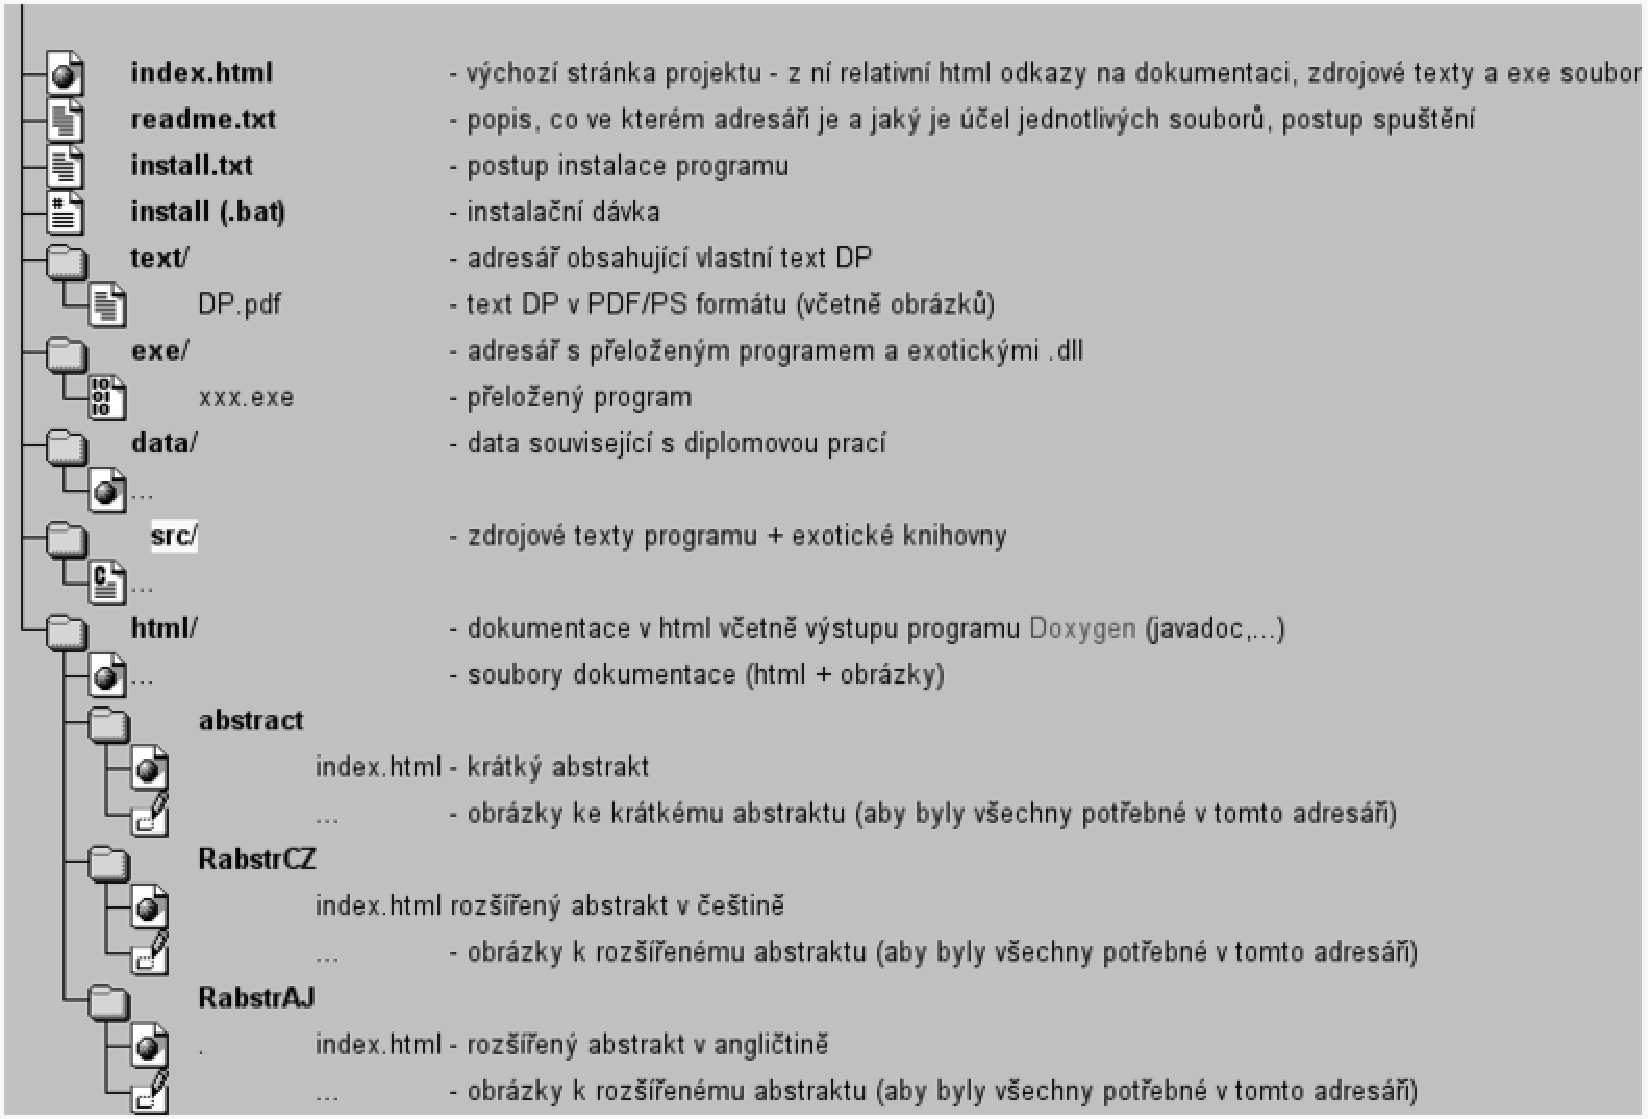
\includegraphics[width=14cm]{figures/seznamcd}
\caption{Seznam přiloženého CD --- příklad}
\label{fig:seznamcd}
\end{center}
\end{figure}
Na GNU/Linuxu si strukturu přiloženého CD můžete snadno vyrobit příkazem:\\ 
\verb|$ tree . >tree.txt|\\
Ve vzniklém souboru pak stačí pouze doplnit komentáře.

Z \textbf{README.TXT} (případne index.html apod.)  musí být rovněž zřejmé, jak programy instalovat, spouštět a jaké požadavky mají tyto programy na hardware.

Adresář \textbf{text}  musí obsahovat soubor s vlastním textem práce v PDF nebo PS formátu, který bude později použit pro prezentaci diplomové práce na WWW.


\end{document}